\documentclass[english,version-2020-11]{uzl-thesis}

% Copy this file as a template for your thesis. You will have to take
% action at all places marked by
%
% !!!!!!!!!!!!!!!!!!!!!!!!!!!!!!!!!!
% !!! Your action is needed here !!!
% !!!!!!!!!!!!!!!!!!!!!!!!!!!!!!!!!!
%
% The first place your action is needed is the first line of this
% document:
%
%
% Language of the thesis:
%
% You must use either 'german' or 'english' above, depending on the
% language used in the main text. This will automatically setup a lot
% of things in the background.
%
%
% Version of the class:
%
% You must specify which version of the thesis class is to be
% used. This is important in case the class style changes in later
% years, but we still want an older thesis to look the same, even when
% things are changed in the class.
%
% Do not change or remove the version-xxxx key.
%
%
% Text encoding:
%
% Your thesis *must* be encoded in utf8 (unicode), which is the
% default in most editors these days. Do *not* change this to latin8.



%%%
%
% Main setup:
%
%%%
%
% You must use the \UzLThesisSetup command to specify numerous things
% about your thesis. This includes the entries on the title page, the 
% abstracts, and the bibliography style. You do so by specifying
% so-called "values" for so-called "keys". For instance, 
% for the key "Autor" you must provide your name as the value. You do
% so by writing 'Autor = {Max Mustermann}', that is, the value is put
% into curly braces. You can use the \UzLThesisSetup command
% repeatedly and the order in which you provide the keys is not
% important. 
%
% Everything shown on the title page must be in German -- even
% if the thesis is written in English! Just insert German text for
% German keys and English text for English keys (like 'Abstract' needs
% English text, while 'Zusammenfassung' needs German text).

\UzLThesisSetup{
  %
  % !!!!!!!!!!!!!!!!!!!!!!!!!!!!!!!!!!
  % !!! Your action is needed here !!!
  % !!!!!!!!!!!!!!!!!!!!!!!!!!!!!!!!!!
  %
  % First, specify the institut or clinic at which the thesis was
  % written. You get the logo file from them (make sure it has the
  % correct size, namely the same as the example). If they do not have
  % a logo, the university's default logo is used.
  %
  % The 'verfasst' gets two arguments. Change the first to {an der}
  % for clinics, as in 'Verfasst = {an der}{Medizinischen Klinik I}'
  %
  Logo-Dateiname        = {uzl-thesis-logo-itcs.pdf},
  Verfasst              = {am}{Institut für Theoretische Informatik},
  %
  % The titles:
  %
  Titel auf Deutsch     = {
     Sichere Steganographie auf ML-Basierten Kanälen (Draft v3)
  }, 
  Titel auf Englisch    = {
    Secure Steganography on ML-Based Channels (Draft v3)
  },
  %
  % Author and supervisor:
  % 
  % Note that the 'Betreuer' or 'Betreuerin' is the supervisor, that
  % is, the professor who officially supervises the thesis. If there
  % is also an assistent of the professor who helped (typically a
  % lot), use 'Mit Unterstützung von' to thank that person. If the
  % thesis was mainly written 'externally' at some company or another
  % institute, point this out using 'Weitere Unterstützung'. 
  % 
  % For your own name, do *not* add things like "BSc" or "BSc
  % cand.". For the supervisor, you should normally include
  % "Prof. Dr." or "PD Dr." (ask your supervisor, what is
  % appropriate), but nothing more (so no
  % "Univ.-Prof. Dr. Dr. h.c. mult." unless your supervisor insists).  
  %
  Autor                 = {Jeremy Boy},
  Betreuer              = {Prof. Dr. Maciej Liśkiewicz},
  % 
  % Optional: Supporting persons and institutions. The text should be
  % in German, even for an English thesis.
  %
%  Mit Unterstützung von = {Harry Hilfreich},
  % 
  %   Weitere Unterstützung = {
  %     Die Arbeit ist im Rahmen einer Tätigkeit bei der Firma Muster GmbH
  %     entstanden.
  %   },
  %
  %
  % Your Degree Programm (Studiengang)
  %
  % Specify 'Bachelorarbeit' or 'Masterarbeit' and the degree
  % programme. Make sure the name of programme is correct and not
  % some abbreviation or some incorrect variant. For instance:
  % 'Medizinische Ingenierwissenschaft', but not 'MIW';
  % 'Medizinische Informatik', but not 'Medizin-Informatik';
  % 'Informatik', but not 'Informatik (SSE)'.
  %
  % Use German names for German programmes and English names for
  % English ones, so 'Infection Biology', not 'Infektionsbiologie'. 
  % For programmes that have a German bachelor and an English master,
  % use the German name for a bachelor thesis and the English name for
  % the master thesis.
  %
  Bachelorarbeit,
  Studiengang           = {IT-Sicherheit},
  %
  % Date on which the thesis is turned in German, formatted the
  % traditional German way:
  %
  Datum                 = {\today},
  %
  % The English abstract. You must always provide abstracts in German
  % and in English. 
  %
  Abstract              = {
    Steganography enables confidential communication even when the use of classical cryptography is prevented or impeded.
    The Meteor stegosystem extends classical steganographic primitives for use on channels based on generative models, such as GPT-2.
    Here, the hiddentext is embedded in the randomness used for sampling from the generative model.
    
    In this thesis, we analyze correctness and security against Chosen-Hiddentext-Attackers of the Meteor stegosystem. 
    We will find that correctness is violated especially for longer hiddentexts ($|m| \geq 1024$ bytes).
    This correctness violation occurs due to ambiguous tokenization of text.
  This can occur with subword tokenization, which is used in modern generative models such as GPT-2.
    Additionally, the Meteor stegosystem is vulnerable to chosen-hidden-text attackers with polynomially many queries.
    We present optimizations that improve the correctness and chosen-hiddentext attack security of the Meteor stegosystem.
    We also discuss a modification that allows Meteor to be used for more compelling use in the context of instant messaging.
  },
  Zusammenfassung       = {
    Steganographie ermöglicht vertrauliche Kommunikation auch dann, wenn die Nutzung klassischer Kryptographie verhindert oder erschwert wird.
    Das Meteor-Stegosystem erweitert klassische steganographische Primitive für die Verwendung auf Kanälen, die auf generativen Modellen basieren, wie etwa GPT-2.
    Hierbei wird der Geheimtext in den verwendeten Zufall im Sampling des generativen Modells eingebettet.
    
    In dieser Thesis werden Korrektheit und Sicherheit gegen Chosen-Hiddentext-Angreifer des Meteor-Stegosystems analysiert. 
    Wir werden feststellen, dass die Korrektheit insbesondere bei längeren Geheimtexten ($|m| \geq 1024$ Bytes) verletzt ist.
    Diese Korrektheitsverletzung tritt aufgrund uneindeutiger Tokenisierung von Text auf.
    Diese kann bei Subword-Tokenisierung, welche in modernen Generativen Modellen wie etwa GPT-2 verwendet wird, auftreten.
    Zudem ist das Meteor-Stegosystem deterministisch und dadurch verwundbar gegen Chosen-Hiddentext-Angreifer mit polynomiell vielen Queries.
    Wir präsentieren Optimierungen, die die Korrektheit und Chosen-Hiddentext-Attack-Sicherheit des Meteor-Stegosystems verbessern.
    Außerdem wird eine Modifikation diskutiert, mit welcher Meteor zur überzeugenderen Verwendung im Kontext von Instant Messaging verwendet werden kann.
  },
  %
  % Optional: 'Danksagungen' (German) or 'Acknowledgements'
  % (English). Both keys are optional and both have the same effect of
  % adding an acknowledgements text after the abstracts and before the
  % table of contents.
  %
  Acknowledgements = {
  First and foremost, I'd like to thank Prof. Dr. Maciej Liśkiewicz for sparking my interest in the topic at hand and allowing me to write this thesis.
  Our meetings and discussions have helped me tremendously to approach and understand the highly exciting topic of steganography.
  
  I also want to thank my parents Viola and Torsten, who always support me on my ways.
  },
  %  This is the place where you can thank people and institutions, do
  %  not try to do this on the title page. The only exception is in
  %  case you wrote your thesis while working or staying at a company or abroad. Then you
  %  should use the \Latex{Weitere Unterstützung} key to provide a text
  %  (in German) that acknowledges the company or foreign
  %  institute. For instance, you could use texts like »Die Arbeit
  %    ist im Rahmen einer Tätigkeit bei der Firma Muster GmbH
  %    entstanden« or »Die Arbeit ist im Rahmen eines
  %    Forschungsaufenthalts beim Institut für Dieses und Jenes an der
  %    Universität Entenhausen entstanden«. Do not name and thank
  %    individual persons from the company or foreign institute on the
  %    title page, do that here. 
  %},
  % Bibliography style: Choose between
  % 
  % 'Alphabetische Bibliographie'
  % for all degree programmes in the natural sciences 
  % 
  % 'Numerische Bibliographie'
  % alternative for all other degree programmes
  % 
  % Either will load biblatex and setup the citation methods and the
  % bibliography styles correctly. You should not mess with them.
  % 
  Alphabetische Bibliographie,
  % Alternatively:
  % Numerische Bibliographie
}


\addbibresource{thesis.bib}


%%%%%%%%%%%%%%%%%%%%
%
% Styling the thesis
%
%%%%%%%%%%%%%%%%%%%%
%
% Creating a visually pleasing layout and choosing fonts is not
% easy. Furthermore, different people have different preferences. Of
% course, for the University of Lübeck, the dean of studies could just
% force everyone to use one specific layout and font, but that seems a
% bit drastic and, also, it seems nice that thesis by different people
% have an individual style even though they all stick to the same
% overall structure.
%
% For these reasons, I (Till Tantau) have spend quite some time on
% designing a flexible layout and styling mechanism for theses.
%
% Basically, the overall structure of the thesis is fixed by the
% thesis class and so are many structural elements. For instance, you
% cannot change the order in which the abstract and table of contents
% are shown, you cannot move the bibliography elsewhere, indeed, the
% bibliography style is also fixed. Likewise, the text on the title
% page is fixed.
%
% Although many things are fixed, you *can* change several other
% things. For instance, you can change the font used for the main
% text, you can change which font is used for titles and headings or
% you can change whether titles and headlines are centered or flushed
% left.
%
% There are many LaTeX packages for changing such things. You are
% kindly asked *not to use them*. Rather, use (only) the options
% offered by the thesis class. All possible choices and combinations
% there have been tested by me and produce nice results; what happens
% with other packages no one knows and might no longer conform to what
% is expected by the university. As you will see, you still have a
% lot of options.
%
%
% Technical note: All styling is done via the command
%
% \UzLStyle{...}
%
% where ... is a key-value list just as for \UzLThesisSetup. The
% difference is just that everything having to do with styling as
% controlled by \UzLStyle, while the more “formal” setup keys are
% controlled by \UzLThesisSetup.
%
%%%
%
% Designs
%
%
% A \emph{design} is a whole set of font and layout options bundled
% together. They have been chosen in such a way that a visually
% pleasing “overall appearance” results.
%
%
% \UzLStyle{computer modern oldschool design}
%
% The look of this design mimics the “classical” way a paper or report
% created with \LaTeX\ looks like: The Computer Modern font is used,
% bold face fonts are used for headlines, only black and white are
% used as colors. This design reminds me of older scientific
% documents, especially from the computer science community where
% \LaTeX\ was used very early.
%
%
% \UzLStyle{computer modern basic design}
%
% A slightly less “oldschool” version of the previous design. It is
% still a classic design in the sense that it uses the Computer Modern
% font and that it still has this “good old \LaTeX” look, but some
% more modern aspects (like colors!) have been added.
%
% Note that this design uses Myriad for the title page (one of the
% “modern aspect”), which means that his font must be installed.
%
%
% \UzLStyle{computer modern scholary design}
%
% In my opinion, this is the ultimate “scholary design”: The thesis
% will look like it has been typeset by hand some 150 years ago and
% then printed by a university press. There is really nothing “modern”
% about it and the word in the name of the design is just part of the
% name of the “Computer Modern” font.
%
%
% \UzLStyle{pagella basic design}
%
% A, well, basic design that uses the Pagella font rather than the
% Computer Modern font. Especially the bold face version of this font
% looks nicer than the Computer Modern counterpart. Also, Pagella,
% while still having a “bookish” look, still feels a bit fresher than
% Computer Modern. 
%
%
% \UzLStyle{pagella centered design}
%
% A variant of the basic Pagella design that centers all
% headlines. A nice alternative to the basic version.
%
%
% \UzLStyle{pagella contrast design}
%
% This design tries to create some visual friction by contrasting the
% sans serif headline font (in bold!) with the main text. I find it a
% visually very interesting combination.
%
%
% \UzLStyle{alegrya basic design}
%
% The third variant of the basic design, this time using the Alegrya
% font. 
%
%
% \UzLStyle{alegrya scholary design}
%
% The Alegrya version of the previous “scholary” design. Unlike the
% Computer Modern version, this design does not look old, but more
% fresh -- while still creating the impression that the text must be
% about a very scientific subject. 
%
%
% \UzLStyle{alegrya stylish design}
%
% The design is quite similar to the scholary version for the Alegrya
% font, but with even more modern additions. “Stylish” is the word
% that comes to my mind.
%
%
\UzLStyle{alegrya modern design}
%
% A design that uses the sans serif version of the Alegrya font for
% the headlines. This is a nice modern overall design.
%
%%%




%%%%%%%%
%
% Now, include the package you need here using \usepackage. 
%
% However, many standard packages are already loaded by the class:
%
% amsmath, amssymb, amsthm, babel, biblatex, csquotes, etoolbox,
% filecontents, fontspec, geometry, hyperref, tikz (with libraries
% arrows.meta, positioning and shapes), varioref, url 
%
% Indeed, in many cases you will not need any extra packages.
%
%%%%%%%

\usepackage{subcaption}
\usepackage[inline]{enumitem}
\usepackage{todonotes}
\usepackage{pgfplots}
\usepackage{msc}

\usepgfplotslibrary{groupplots}

\renewcommand{\chapterautorefname}{Chapter}
\renewcommand{\sectionautorefname}{Section}
\renewcommand{\theoremautorefname}{Definition}
\newcommand{\definitionautorefname}{Definition}
\newcommand{\lstlistingautorefname}{Listing}

\newcommand{\exampleref}[1]{Example \ref{#1}}

\newcommand{\leftarrowS}{\mathrel{{\leftarrow}\vcenter{\hbox{\scriptsize\rmfamily\upshape\$}}}}

\begin{document}

\chapter{Introduction}

\section{Motivation}

When governmental or private-sector adversaries try to breach the confidentiality of private communication, society requires means to defend their privacy.
Especially in authoritarian states, law enforcement continuously attempts to break or prohibit effective means of cryptography \cite{TLSBlocking2020}.

Steganography extends the concepts of cryptography by not only hiding the contents of a message, but also hiding the mere existence of a hidden message.
If we are able to establish provably secure steganographic protocols -- or stegosystems -- people can use them to circumvent censorship and avoid persecution in hostile environments.
Steganographic techniques are already in use today, for example in the Tor anonymity service to circumvent the so-called ``Great Firewall'' of China \cite{TorBlocking2012}.

This thesis discusses Meteor, an innovative steganographic protocol that exploits the randomness used in sampling from distributions of machine learning based text generation models such as GPT-2 to embed a hidden message into the generated text.
We will show that the Meteor stegosystem is not reliable with regard to the formal definition of steganographic reliability.
Afterwards, we present a modification to the Meteor stegosystem to improve its use in instant messaging applications by replacing the generative model with one that is primed to generate chat-like texts.
Subsequently, Meteor's security against chosen hiddentext attackers is discussed.
We will discuss that an attacker can distinguish Meteor's output from a random oracle in polynomial queries.
For both reliability and security, algorithms are presented that improve the Meteor stegosystem.


\section{Structure of this Thesis}

\autoref{chap:preliminaries} introduces notation that will be used throughout this thesis.

\autoref{chap:previous-work} discusses previous works we will need to understand the architecture of the Meteor stegosystem.
First, we will discuss steganography and provably secure steganography as defined in \cite{Hopper2004}.
Afterwards, we discuss how generative neural networks such as GPT-2 iteratively produce high-quality text.
Concluding, the Meteor stegosystem is presented, a provably secure steganographic system over ML-based channels as introduced in \cite{Meteor2021}.

\autoref{chap:reliability} analyzes the reliability of the Meteor stegosystem. 
This chapter relies on the material presented in \autoref{chap:previous-work}, especially the definitions of steganographic (un-)reliability established in \autoref{def:unreliability} and \autoref{def:reliability} as well as the discussion of generative neural networks (GNNs) in \autoref{sec:generative-neural-networks}.
We will see that the Meteor stegosystem is not reliable because of subword tokenization used in most modern GNNs.
Afterwards, algorithms are presented that improve reliability of Meteor on the receiver site.
Unfortunately, these algorithms -- in the worst case and for some models -- introduce overhead exponential in the length of the generated stegotext.

In \autoref{chap:twowaycommunication} we present a small modification to the Meteor stegosystem that allows two-way communication.
This chapter relies on the material presented in \autoref{sec:meteor} and \autoref{sec:generative-neural-networks}.
There, we embed a fixed amount of bits in each message, using the DialoGPT model presented in \cite{Zhang2020} to generate dialog-like messages.
This modification allows users of the Meteor stegosystem to communicate more naturally in the context of instant messaging.
It also makes sure that the algorithms from \autoref{chap:reliability} can be applied more conveniently with smaller overhead.

In \autoref{chap:security}, we will perform a security analysis of the Meteor stegosystem using Hopper's definition of a secure stegosystem.
This chapter relies heavily on the material presented in \autoref{chap:previous-work}, especially the security definitions in \autoref{def:sec-hopper} and \autoref{def:sec-kaptchuk}.
We will compare the definition of security used by the Meteor authors with the definition of security by Hopper.
We will then show that the Meteor stegosystem is not secure with regard to Hopper's definition.
Afterwards, a modification to the Meteor stegosystem is presented that increases its security against chosen hiddentext attackers.

Finally, in \autoref{chap:conclusion}, we will discuss the results and propose topics for further research in a conclusion.

\chapter{Preliminaries}
\label{chap:preliminaries}
In this chapter, we will introduce the notation that will be used in this thesis.

We denote by $x \leftarrowS S$ a value $x$ sampled uniformly at random from the set $S$.
We denote the power set of $S$ by $2^S$.

When working with a probability distribution $D$, $x \leftarrowS D$ denotes the random sampling of a value according to $D$.
We also denote the probability of some value $x \in D$ as $Pr_D[x]$ or $Pr[x]$ if the distribution is clear from context.
We define $U_n$ as the uniform distribution over bit strings of length $n$.

In code samples, we denote $x \leftarrow a$ as assignment of value $a$ to variable $x$.
When working with sorted sequences, such as arrays or strings, we use pythonic slicing notation.
Given a sequence $x = (x_0, x_1, \dots, x_{n-1})$ of length $n$, we use the following slicing operations:

\begin{itemize}
  \item $x[i] = x_i$,
  \item $x[i:j] = (x_i, x_{i+1}, \dots, x_{j-1})$,
  \item $x[i:] = x[i:n] = (x_i, x_{i+1}, \dots, x_{n-1})$.
\end{itemize}

We use $x \leftarrow \epsilon$ as the empty value assignment.
We also use the infix operator $\oplus \colon \{0,1\}^n \times \{0,1\}^n \rightarrow \{0,1\}^n,~ a \oplus b$ for the exclusive-or of values $a$ and $b$.
The infix concatenation operator $|| \colon X^n \times X^m \rightarrow X^{n+m},~ a||b$ appends the value or sequence $b$ to $a$. 

The variable $\lambda$ denotes the security parameter used in cryptographic primitives or steganographic protocols.
We denote by $\mu(\lambda)$ a function negligible in $\lambda$, i.e., for every integer $c$ there exists an integer $c_0$ such that for all $\lambda > c_0$,
$$|\mu(\lambda)| < \frac{1}{\lambda^c}.$$

In general, the hiddentext in a steganographic protocol is a bit string $m \in \{0,1\}^*$.
In this thesis, however, we use sequences of Unicode characters as hiddentexts.
We denote the set of Unicode characters as $\mathcal{U}$ and hiddentext messages $m \in \mathcal{U}^*$ as strings of Unicode characters.

\chapter{Background of the Meteor Stegosystem}
\label{chap:previous-work}

\section{Provably Secure Steganography}
\label{sec:prov-sec-steg}

Steganography extends the concepts of cryptography to hide the mere existence of a message.
This makes it robust against censorship and prohibition.
While cryptography can be used to hide the contents of a confidential message, its use is easily discoverable by adversaries.


Steganography is usually modeled using the Prisoners' Problem, as introduced in \cite{Simmons1983}.
The participants Alice and Bob are imprisoned.
While they can exchange messages, their contents are surveilled by a warden we will call Eve.
Alice and Bob now want to craft and exchange escape plans while Eve observes the messages exchanged between Alice and Bob.
Since Eve does not want Alice and Bob to leave the prison prematurely, she tries to distinguish the exchange of the escape plan from innocuous messages.
If Eve succeeds, she suppresses the message.
For an illustration of the Prisoners' Problem see \autoref{fig:prisonersgame}.

\begin{figure}[htbp]
\centering
\begin{tikzpicture}
	\node[block] (alice) {Alice};
	\node[block, right=3cm of alice] (warden) {Eve};
	\node[block, right=3cm of warden] (bob) {Bob};
	\node[left=of alice] (m) {$m$};
	\node[above=of alice] (k) {$k$};
	\node[below=of alice] (h) {history $h$};
	\node[right=of bob] (mb) {$m$};
	\node[above=of bob] (kb) {$k$};
	\node[below=of bob] (hb) {history $h$};
	\node[block, below=of warden] (steganalysis) {Steganalysis: is $s$ stegotext?};
	\node[below left=of steganalysis] (isstego) {suppress message};
	\node[below right=of steganalysis] (notstego) {forward message to recipient};
	\draw[->] (alice) -- node[above] {$s$} (warden);
	\draw[->] (warden) -- node[above] {$s$} (bob);
	\draw[->] (m) -- (alice);
	\draw[->] (k) -- (alice);
	\draw[->] (h) -- (alice);
	\draw[->] (bob) -- (mb);
	\draw[->] (kb) -- (bob);
	\draw[->] (hb) -- (bob);
	\draw[->] (warden) -- (steganalysis);
	\draw[->] (steganalysis) -- node[below] {Yes} (isstego);
	\draw[->] (steganalysis) -- node[below] {No} (notstego);
\end{tikzpicture}
\caption{
An illustration of the Prisoners' Problem \cite{Simmons1983}.
Two accomplices in a crime (Alice and Bob) are imprisoned in widely separated cells.
They want to escape and try to coordinate their escape plans.
They are surveilled by a warden Eve who monitors their communication.
If Eve detects a hidden message by successfully distinguishing it from an innocuous message, she suppresses the message.
Otherwise, the message is forwarded.
It is expected that Alice and Bob have been able to exchange a secret key $k$.
They also have access to the same initial history $h$, which can be public.
}
\label{fig:prisonersgame}
\end{figure}

While the Prisoners' Problem has already been established in the 1980s, the cryptographic community was lacking a strict definition of steganographic secrecy until the early 2000s.
In \cite{HLA2002}, a steganographic protocol based on rejection sampling is presented, the first known example of a general provably secure steganographic system.
On the way, the authors also establish a cryptographic point of view on steganographic channels and steganographic protocols as well as the notion of steganographic secrecy against chosen hiddentext attackers.
The definitions and theorems established by Hopper, Langford and von Ahn have succeedingly been advanced in Hopper's dissertation \cite{Hopper2004} and further works by other researchers.

\begin{definition}[Channel, \cite{Hopper2004}, \cite{Wölfel2011}]
Let $\Sigma = \{0,1\}^\sigma$ be a finite set of bit-strings, or \emph{documents}, of length $\sigma$.
$\Sigma^\ell$ denotes the set of \emph{sequences} of length $\ell$ of bit-strings over $\Sigma$, and $\Sigma^*$ the set of sequences of finite length over $\Sigma$.

A \emph{channel} $\mathcal{C}$ is a function that takes a history $h \in \Sigma^*$ as input and produces a probability distribution $\mathcal{D}_{\mathcal{C},h}$ on $\Sigma$.
We denote the set of histories for $\mathcal{C}$ as $\mathcal{H}$.
\end{definition}

A sequence $s = s_1||s_2||\dots||s_\ell \in \Sigma^\ell$ of documents can be generated by repeatedly generating the distribution $\mathcal{D}_{\mathcal{C},h||s_1||s_2||\dots||s_i}$ by querying $\mathcal{C}$ with some initial history $h$ and appending the value sampled from the distribution to $h$.
We will now formally introduce the notion of \emph{marginal channel distribution}, which we will later need for the definition of steganographic secrecy.

\begin{definition}[Marginal Channel Distribution, \cite{Hopper2004}]
Let $\mathcal{C}$ be a channel over $\Sigma$ and $h \in \mathcal{H}$ a history.
We let $\mathcal{C}_h = \mathcal{D}_{\mathcal{C},h}$ denote the \emph{marginal channel distribution on a single document from $\Sigma$} conditioned on the history $h$ of already drawn documents.
We let $\mathcal{C}_h^\ell$ denote the \emph{marginal channel distribution on a sequence of $\ell$ documents} from $\Sigma$ conditioned on the history $h$ of already drawn documents.
\end{definition}
%We will also need the notion of an \emph{always informative channel}.
%An always informative channel is a channel with minimum-entropy bounded by some value $\alpha$.
We will also need the notion of the \emph{support of a distribution}.
The support of a distribution consists of all elements with non-zero probability.

\begin{definition}[Support]
Let $D$ be a distribution.
We denote the \emph{support of $D$} as 
$$\mathop{supp}(D) = \{ x \in D \colon Pr_{D}[x] \neq 0 \}$$
\end{definition}

Now that we have established the notion of channels, we can commence with the definiton of a stegosystem.

\begin{definition}[Stegosystem, \cite{Hopper2004}]
\label{def:stegosystem}
A \emph{steganographic protocol} $\mathcal{S}$, or \emph{stegosystem}, with security parameter $\lambda$ is a pair of probabilistic algorithms:

\begin{itemize}
	\item $\mathcal{S}$.Encode (abbreviated $SE$) takes as input a key $k \in \{0,1\}^\lambda$, a string $m \in \{0,1\}^*$ (the hiddentext), and a message history $h \in \mathcal{H}$.
		$SE(k, m, h)$ returns a sequence of documents $s_1||s_2||\dots||s_l$ (the stegotext) from the support of $\mathcal{C}_h^l$.
	\item $\mathcal{S}$.Decode (abbreviated $SD$) takes as input a key $k \in \{0,1\}^\lambda$, a sequence of documents $s_1||s_2||\dots||s_l$, and a message history $h \in \mathcal{H}$.
		$SD(k, s, h)$ returns a hiddentext $m \in \{0,1\}^*$
\end{itemize}
\end{definition}

This definition resembles that of a symmetric encryption scheme, except that both $SE$ and $SD$ take a message history $h$ as additional argument.
Now that we have defined what a steganographic protocol is, we will introduce some properties we would like a stegosystem to satisfy.
First of all, we want a stegosystem to be correct.
The decoding of a given stegotext $s$, given the correct key $k$ and history $h$, should yield the original hiddentext $m$.
Hopper defines the correctness of a stegosystem as follows:

\begin{definition}[Correctness, \cite{Hopper2004}]
\label{def:correctness-hopper}
A stegosystem $\mathcal{S}$ is \emph{correct} if for every polynomial $p(\lambda)$, there exists a negligible function $\mu(\lambda)$ such that $SE$ and $SD$ satisfy the following relationship, where the randomization is over the key $k$ and any coin tosses of $SE$, $SD$, and the oracles accessed by $SE$, $SD$.

$$\forall m \in \{0,1\}^{p(\lambda)},~ h \in \mathcal{H} \colon Pr[SD(k, SE(k, m, h), h) = m] \geq 1 - \mu(\lambda)$$

\end{definition}

The introduction of a \emph{negligible function} $\mu(\lambda)$ allows the stegosystem to sometimes yield wrong results, but only with probability negligible in the security parameter $\lambda$.
While there might be stegosystems with $\mu(\lambda) = 0$, the introduction of a negligible function proves helpful for reductions on established cryptographic primitives.

Since we naturally want our stegosystem to be prone to analysis by Eve, we also need a definition of security.
Intuitively, we want Eve to be unable to efficiently detect the use of a stegosystem $\mathcal{S}$ without knowledge of the secret key $k$.
To show that Eve cannot detect the use of $\mathcal{S}$, we establish an oracle $\mathcal{O}$ which does not actually use $SE$ to encode a hidden message $m$, but instead draws a random sequence of documents of length $|SE(k,m,h)|$ from $\mathcal{C}$.
If Eve is allowed to choose the hiddentext $m$ and history $h$, we call her a \emph{chosen hiddentext attacker}.

We can model this attack as a distinguishing game between a challenger and the adversary Eve.
First, the challenger samples a key $k \leftarrowS U_\lambda$.
Next, Eve sends a tuple $(m, h)$ to the challenger.
The challenger now secretly flips a coin.
If the coin shows heads, the challenger uses $SE$ to generate a stegotext $s = SE(k,m,h)$.
Otherwise, the challenger uses $\mathcal{O}$ to generate a covertext $s$.
Either way, the challenger sends $s$ back to Eve.
If Eve is able to guess the result of the coin flip using a distinguisher $W$, she must have been able to distinguish a stegotext from a covertext.

If Eve can distinguish a stegotext from a covertext, we say that she has an advantage against the stegosystem in the distinguishing game.
The naïve approach to win this game would be to simply guess the coin flip with a success rate of $\frac{1}{2}$ if they play this game just once.
The challenger and Eve repeat this game $q(\lambda)$ times with up to $l(\lambda)$ bits of hiddentext chosen by Eve.
Additionally, Eve is limited computationally by time $t(\lambda)$.
The insecurity of a stegosystem is the maximum possible advantage any attacker can have.
Formally, Hopper defined a chosen hiddentext attack as follows:

\begin{definition}[Chosen Hiddentext Attack, \cite{Hopper2004}]
In a chosen hiddentext attack, $W$ is given access to a ``mystery oracle'' $M$ which is chosen from one of the following distributions:

\begin{enumerate}
\item $ST$: The oracle $ST$ has a uniformly chosen key $k \leftarrowS U_\lambda$ and responds to queries $(m, h)$ with a stegotext drawn from $SE(k, m, h)$.
\item $CT$: The oracle $CT$ has a uniformly chosen $k$ as well, and responds to queries $(m, h)$ with a covertext of length $\mathcal{l} = |SE(k, m, h)|$ drawn from $\mathcal{C}_h^{\mathcal{l}}$
\end{enumerate}

$W^M(1^\lambda)$ outputs a bit which represents its guess about the type of $M$.
We define $W$'s \emph{advantage against a stegosystem $\mathcal{S}$ for channel $\mathcal{C}$} by

$$Adv_{\mathcal{S}, \mathcal{C}, W}^{ss}(\lambda) = |Pr[W^{ST}(1^\lambda)=1] - Pr[W^{CT}(1^\lambda)=1]|$$

where the probability is taken over the randomness of $ST$, $CT$, and $W$. 
Define the \emph{insecurity of $\mathcal{S}$ with respect to channel $\mathcal{C}$} by

$$InSec_{\mathcal{S}, \mathcal{C}}^{ss}(t, q, l, \lambda) = \max_{W \in \mathcal{W}(t, q, l)} \left\{ Adv_{\mathcal{S}, \mathcal{C}, W}^{ss}(\lambda) \right\}$$

where $\mathcal{W}(t, q, l)$ denotes the set of all adversaries which make at most $q(\lambda)$ queries totaling at most $l(\lambda)$ bits (of hiddentext) and running in time at most $t(\lambda)$.
\end{definition}

\begin{definition}[Steganographic Secrecy, \cite{Hopper2004}]
\label{def:sec-hopper}
A Stegosystem $\mathcal{S}$ with security parameter $\lambda$ is called \emph{$(t,q,l,\epsilon)$ steganographically secret against chosen hiddentext attack for the channel $\mathcal{C}$} ($(t,q,l,\epsilon)$-SS-CHA-$\mathcal{C}$) if $InSec_{\mathcal{S},\mathcal{C}}^{ss}(t,q,l,\lambda) \leq \epsilon$
\end{definition}

In the past two decades, many researchers built upon those cryptographic definitions of steganographic protocols.
In \cite{DIRR2008}, complexity limitations of black-box steganography were investigated.
In black-box steganography the sending party Alice knows nothing about the underlying distribution except a bound to its min-entropy and the ability to sample from it (but does not have to know the generated distribution) while Bob needs no access to the channel at all.
While a black-box construction provides a definition with the least required knowledge of the channel, exponential sampling complexity is required for the encoding party with respect to the number of message bits.

In contrast, white-box steganography describes the other extreme, where Alice either knows the channel distribution beforehand or can efficiently compute it.
Both black-box and white-box steganography are unrealistic in practice, because Alice is possibly able to gain some knowledge or approximation about the channel, but most of the time cannot perfectly describe the channel's distribution.
Therefore, grey-box steganography has been introduced \cite{LRW2013}.
Grey-box steganography tries to resolve these deficiencies by expecting that Alice has some initial knowledge of the covertext channel.
Alice then uses machine learning techniques to learn about the covertext distribution and generates suitable stegotexts.
This allows the use of steganography on efficiently learnable covertext channels and lowers the required complexity to sample stegotext documents.

\section{Generative Neural Networks}
\label{sec:generative-neural-networks}

Generative Neural Networks (GNN) establish a model which approximate realistic distributions such as natural language.
In the last years the artificial intelligence community achieved tremendous progress in building powerful models based on deep learning, which was proposed in \cite{DeepLearning2015}.

One of the milestones in deep learning based generative models certainly is the development and release of the Generative Pretrained Transformer, or GPT \cite{OpenAI2018}.
Its successors GPT-2 \cite{OpenAI2019} and GPT-3 \cite{OpenAI2020} quickly became two of the industry-standard models in the natural language processing (NLP) community.
While the GPT-n family is mostly known for its capabilities in text generation, it is not specifically designed to generate blog posts or newspaper articles.
It can also be used for a variety of other NLP tasks, such as question answering, sentiment detection or automatic text summarization.
While GPT-3 can only be used via a paid online API, GPT-2 has been open-sourced in 2019 \cite{GPTReleasePlan2019}.
This makes GPT-2 ideal for use in research.

All members of the GPT-n family are attention-based transformer models, which were introduced in \cite{Vaswani2017}.
Before transformers, state of the art machine learning models were often built using recurrent neural networks (RNNs) such as the long-short-term memory model, or LSTM \cite{Hochreiter1997}.

In comparison to RNNs, transformer models are able to achieve significantly higher training and prediction performance.
While both RNNs and transformer models parse their inputs as a vector of so-called tokens, they differ in the way they process them to generate an output.
In RNN, the input tokens are parsed one word at a time, while transformer models are able to parse all input tokens at the same time.
This is due to the architecture of RNNs.
RNNs consist of a loop structure that parses one input token after the other together with a hidden state vector and outputs a hidden state vector for the next iteration.

A transformer model, on the other hand, uses attention and refrains from using a hidden state vector like RNNs do.
Instead, for each output token, the transformer model weighs its attentions on the input, where the sum of attention weights $\omega_i$ over an input of length $n$ must add up to $\sum_{1\leq i \leq n} \omega_i = 1$.
This technique mimics the way human attention works.
For example, when translating a sentence from one language to another, the translator puts their attention to different parts of the input to determine the correct output word at a given position.

\begin{example}[Example of LSTM and attention in translation]
	When translating the english sentence ``The cat likes to eat bananas very much.'' to german ``Die Katze isst sehr gerne Bananen.'', the structure of the output differs significantly from that of the input.
	In an RNN, the model has to remember the token ``eat'' until the token ``isst'' is generated.
	This information has to be encoded in the hidden state vector while parsing the input and be carried throughout the output generation.
	Since each output in the RNN alters the hidden state, the translation has to performed in a serial manner.
		
	In contrast, a transformer model uses attention at each step of output generation.
	When generating the token ``isst'', the models attention will predominantly be weighed to the input token ``eat'', but some attention will also be placed on ``likes'' and ``the cat'' to produce a grammatically correct sentence.
	Meanwhile other tokens such as ``very'' will have low attention since that word is not relevant to generate ``isst''.
\end{example}



When we use GPT-2 in the Meteor stegosystem, we can abstract its prediction functionality as a function $\mathcal{GPT} \colon \mathcal{T}^\zeta \rightarrow \mathbb{Z}^{|\mathcal{T}|}$.
It takes an input vector $v \in \mathcal{T}^\zeta$ of tokens (with $\zeta$ the history length supported by the model) and transforms it into a logits vector of unweighted model outputs (the next token prediction) of dimension $|\mathcal{T}|$.

The input vector $v=T(h)$ is a representation of a history $h$ generated using a tokenizer $T$ over tokens $\mathcal{T}$.
Since we work with text, we need to find a way for $T$ to transform our history $h$ into the realm of numbers, i.e. tokenize the history.
To do that, we use a set of tokens $\mathcal{T} = \{ t_1, t_2, \dots, t_\ell \}$ specific to the model.
In the simplest case, the tokens can be the characters of the english language, i.e. $\mathcal{T} = \{ a, b, \dots, z, A, B, \dots, Z, 0, 1, \dots, 9, \textrm{'}, ", \dots \}$.
We can then encode a string $h$ with $|h| \leq \zeta$ as a vector $v = T(h) \in \mathcal{T}^{|h|}$, fill the remaining $\zeta - |h|$ entries in the vector with a special padding token $\epsilon$ and pass it to $\mathcal{GPT}$.
	
While the character based approach could work, it is hard for the model to learn the relationship between words solely on the sequence of characters, which badly influences the quality of outputs.
Are ``do'' and ``don't'' more closely related then ``do'' and ``to''?
Probably yes.
But on the character level, ``do'' and ``to'' are very close to each other as they only differ in one character.
Meanwhile, ``do'' and ``don't'' share a common prefix, but differ in three characters (if we pad ``do'' with padding token $\epsilon$).
As we can see, the disadvantages of character based tokenization are long token sequences and meaninglessness of each token for itself.

We could also use words of the english language as tokens, where each word is represented by a unique token.
But this results in large token sets.
It is also unlikely that any token set of full words can be exhaustive for all kinds of texts, especially if we take typographical errors or neologisms into account.
Also, word based tokenization makes it hard for a machine learning algorithm to learn relationships between words.
Similar words -- such as the examples ``do'' and ``to'' from above -- can have vastly different meanings, while the mistyped word ``bananna'' probably means the same as ``banana''.

To tackle the challenges of natural language, most modern text generation models use subword tokenization.
Subword tokenization uses encoding techniques to find common sequences of characters and establishes these as tokens.
One of the commonly used encoding techniques in NLP (and coincidentally the one used in the GPT-n family) is byte-pair encoding (BPE), which was originally introduced as a data compression algorithm in \cite{BPE1994} and proposed as an encoding algorithm in neural machine translation in \cite{BPENMT2016}.
With subword tokenization, a token may not only be a single character or a full word of a given language, but also a substring of a word.
The use of subword tokens allows a model to better predict relationships between words.
For example, the words ``do'' and ``don't'' are probably closely related.
With subword tokens, a tokenizer can parse ``don't'' as ``do$||$n't''. 
An NLP model might then learn that the token ``n't'' can be used to negate a verb.
While this approach makes it easier for the model to learn relationships between different words, there may exist multiple tokenizations for a given word, a pitfall that will be important when we discuss correctness in \autoref{chap:correctness}.

After the tokenizer has encoded the history as a vector of tokens it is passed as input to the generative model.
The model's output is a logits vector $z \in \mathbb{Z}^{|\mathcal{T}|}$ with components $z_i$ for each token $t_i$ in the model's token set.
A logits vector is a vector of unweighted activations of the model's underlying layers, where a higher value in a component represents a stronger activation and therefore a higher likelyhood of a token to appear as the next token in the sequence.
Since the logits vector is unweighted, it might contain positive and negative values, which don't sum up nicely as they would in a probability distribution we can sample from.
To get a probability distribution from a logits vector $z \in \mathbb{Z}^{|\mathcal{T}|}$ we can use the softmax function $\sigma$, which transforms a logits vector of some dimension $\ell$ into another vector of the same dimension representing the probability mass function for the components of the logits vector:

$$\sigma \colon \mathbb{Z}^{\ell} \rightarrow [0,1]^{\ell},~ \sigma(z) = \left(\frac{e^{z_i}}{\sum_{j=1}^{\ell} e^{z_j}}\right)_{1 \leq i \leq \ell}$$

When we combine all the previous steps, we get the black box for our ML model as illustrated in \autoref{fig:generative-network}.

\begin{figure}[htpb]
	\centering
	\begin{tikzpicture}
            \node[rectangle, draw=black, minimum width=4cm, minimum height=4cm] (oracle) {$\mathcal{GPT}$};
            \node[right=of oracle, rectangle, draw=black, minimum width=2cm, minimum height=4cm] (sigmoid) {$\sigma$};
            \node[left=of oracle, rectangle, draw=black, minimum width=2cm, minimum height=2cm] (transform) {Tokenizer};
            \node[left=of transform] (history) {$h$};
            \node[above right=-5mm and 1.2cm of sigmoid] (t1) {$t_1$};
            \node[below=5mm of t1] (t2) {$t_2$};
            \node[below=5mm of t2] (t3) {$t_3$};
            \node[below=5mm of t3] (t4) {$\dots$};
            \node[below=5mm of t4] (tn) {$t_{|\mathcal{T}|}$};
            \node[draw,dashed,inner sep=2mm,label={$Next_{\mathcal{GPT}}$},fit=(sigmoid) (oracle) (transform)] {};
            \draw[->] (transform) -- node[midway,above] {$v$} (oracle);
            \draw[->] (history) -- (transform);
            \draw[->] (oracle) -- node[midway,above] {$z$} (sigmoid);
            \draw[->] (sigmoid) -- node[midway,below] {$p_1$} (t1);
            \draw[->] (sigmoid) -- node[midway,below] {$p_2$} (t2);
            \draw[->] (sigmoid) -- node[midway,below] {$p_3$} (t3);
            \draw[->] (sigmoid) -- node[midway,below] {$p_{|\mathcal{T}|}$} (tn);
	\end{tikzpicture}
	\caption{
Generative ML Model as a pipeline $Next_{\mathcal{GPT}}$ as it is used in the Meteor stegosystem, which takes as input a history $h \in \mathcal{H}$ and outputs a tuple $(\mathcal{T}, \mathcal{P})$, where $\mathcal{P} = \{p_1, p_2, \dots, p_{|\mathcal{T}|}\}$ is a probability distribution over tokens $\mathcal{T} = \{ t_1, t_2, \dots, t_{|\mathcal{T}|}\}$. 
The history $h$ is a string of text which is transformed to a vector $v \in \mathcal{T}^\zeta$ (with model-specific $\zeta$) of token indices using a tokenizer.
The prediction model $\mathcal{GPT}$ takes $v$ as input and returns a logits vector $z \in \mathbb{Z}^{|\mathcal{T}|}$ of unscaled outputs.
This logits vector is then transformed to a probability distribution $p \in [0,1]^{|\mathcal{T}|}$ using the softmax function.
	The component $p_i$ represents the probability of token $t_i \in \mathcal{T}$ to be the next token in the sequence $s$ given the history $v$ of length $\zeta$: $p_i = Pr[s_{\zeta+1}=t_i|s=v]$.
}
	\label{fig:generative-network}
\end{figure}

\todo{fix alignment of $p_{|\mathcal{T}|}$}

To generate the next token in the sequence, we can sample according to the generated distribution.
After sampling from the distribution, we append the sampled token to the history and repeat the process until sufficiently many tokens have been generated.
We then convert the token outputs to a string using the tokenizer to get the generated text.
For an example of GNN model outputs using GPT-2, see \exampleref{example:gpt2-output-sample}.

\begin{example}[Example of GPT-2 model output for initial history ``What is steganography in computer science?'']
It is a form of digital communication that uses data to hide or obscure messages from a third party. It has become so common that today it is one of the most popular ways of communicating online. Steganography can be used to send photos or videos to another user or to hide messages from someone who will not discover the sender is actually the sender. As a result, it has become a real phenomenon known as "steganography".
	\label{example:gpt2-output-sample}
\end{example}

To use GPT-2 with the Python programming language, we can use the Hugging Face Transformers library together with PyTorch.
PyTorch \cite{PyTorch} is a machine learning framework that implements high performance operations needed for machine learning with support for hardware acceleration.
The Hugging Face Transformers library \cite{HFTransformers} is built upon PyTorch and gives an API for easy access to several pretrained machine learning models.
In its simplest form, the pipeline API generates texts using not only GPT-2 but many other generative models.
A Python program which generates the text in \exampleref{example:gpt2-output-sample} can be found in \autoref{alg:gpt2-demo}.

While the use of the pipeline API is very convenient to develop simple text generation or question answering programs, it abstracts some steps that we will need to intercept for use in a stegosystem.
A more sophisticated way to generate text using GPT-2 can be found in \autoref{alg:gpt2-logits-demo}.
Its output resembles that shown in \exampleref{example:gpt2-output-sample}. 
This code example shows how we can:

\begin{itemize}
	\item use a tokenizer to convert strings to a vector of tokens
	\item use the model to get a logits vector
	\item transform a logits vector into a probability mass function using the softmax function
	\item sample the next token from the distribution
	\item convert a vector of tokens back to a string using the tokenizer
\end{itemize}

As we can see in \autoref{alg:gpt2-logits-demo}, a pseudorandom value \emph{sample} is generated to select the next token \emph{selection} from the distribution.
This is what the Meteor stegosystem will abuse.
There, the sending party will replace the randomness with a crafted value to embed a hidden message.
While that value seems random to an observer, a recipient who possesses the secret key is able to recover the hidden message.


\lstinputlisting[style=code, language=Python, caption={Python text generator using the Hugging Face Transformers Pipeline API}, label={alg:gpt2-demo}]{code/pipeline_gpt2.py}

\lstinputlisting[style=code, language=Python, caption={Python text generator using the Hugging Face Transformers library}, label={alg:gpt2-logits-demo}]{code/logits_demo_gpt2.py}

\newpage

\section{Meteor Stegosystem}
\label{sec:meteor}
In their paper \cite{Meteor2021}, the authors present the Meteor stegosystem, a provably secure steganographic system for realistic distributions approximated by ML models.
The central idea behind Meteor is that an encoding party Alice manipulates the randomness used in a sampling scheme to embed hidden text in a token sequence.
The decoding party Bob receives the generated stegotext from Alice and recovers a prefix of the random value used during sampling.
If the value which replaces the randomness for sampling is indistinguishable from an actually random value, the steganographic protocol is secure.

While it is easily possible for the encoding party to manipulate the sampling because they control the randomness, it is intuitively unclear whether the decoding party can extract a prefix of the randomness from the stegotext to recover parts of the hiddentext message.
Luckily, with many generative neural networks, such as GPT-2, the decoding party can do that.
The Meteor authors have introduced the concept of Ranged Randomness Recoverable Sampling Schemes, or RRRSS.
This definition formally models the desired behavior described above.

\begin{definition}[Ranged Randomness Recoverable Sampling Scheme, \cite{Meteor2021}]
	\label{def:rrrss}
	We call 
	$(Sample_{\mathcal{D}}^\beta, Recover_{\mathcal{D}}^\beta, \mathcal{D}, \beta, \mathcal{H})$ 
	with ppt. algorithms
	$Sample_{\mathcal{D}}^\beta \colon \mathcal{H} \times \{0,1\}^\beta \rightarrow \Sigma$ 
	and 
	$Recover_{\mathcal{D}}^\beta \colon \mathcal{H} \times \Sigma \rightarrow \mathcal{P}(\{0,1\}^\beta)$ 
	a \emph{Ranged Randomness Recoverable Sampling Scheme} (RRRSS) over distribution $\mathcal{D}$ with precision $\beta \in \mathbb{N}$ and histories $\mathcal{H}$, if:
	
	\begin{enumerate}
		\item $Sample_{\mathcal{D}}^\beta(h, r)$ on history $h \in \mathcal{H}$ and randomness $r \in \{0,1\}^\beta$, sample an output $s$ from the underlying distribution $\mathcal{D}$
		\item $Recover_{\mathcal{D}}^\beta(h, s)$ on history $h \in \mathcal{H}$ and sample $s \in \Sigma$ returned from $Sample_{\mathcal{D}}^\beta$, output the set $\mathcal{R} = \{ r \in \{0,1\}^\beta | Sample_{\mathcal{D}}^\beta(\mathcal{H}, r) = s \}$ of possible values for $r$
	\end{enumerate}
\end{definition}

With the definition of an RRRSS, the authors define sampling and recovery algorithms for the GPT-2 model.
While they define the $Sample$ and $Recover$ algorithms for GPT-2 only, they argue that many generative models satisfy the RRRSS property.

\begin{Pseudocode}[caption={
RRRSS $Sample$ algorithm for GPT, \cite{Meteor2021}.
$Sample$ produces, given a history $h$ and a value $r$, the next token sampled according to $r$ from the distribution for the next token generated by $Next_{\mathcal{GPT}}(h)$.
}]
algorithm $Sample_{\mathcal{GPT}}^\beta(	h, r)$
	Output: Token $t$
	$\mathcal{T}, \mathcal{P} \leftarrow Next_{\mathcal{GPT}}(h)$
	$cuml \leftarrow 0$
	for $i \in \{ 0, 1, \dots, | \mathcal{T} - 1 | \}$ do
		$cuml \leftarrow cuml + \mathcal{P}[i]$
		if $cuml > r$ then
			Output $t \leftarrow \mathcal{T}[i]$
	Output $t \leftarrow \mathcal{T}[|\mathcal{T}|-1]$
\end{Pseudocode}

\begin{Pseudocode}[caption={
RRRSS $Recover$ algorithm for GPT, \cite{Meteor2021}.
Given a history $h$ and a sample $s$, return a set of possible random values used to generate $s$ with history $h$.
}]
algorithm $Recover_{\mathcal{GPT}}^\beta(h, s)$
	Output: Randomness set $\mathcal{R}$
	$\mathcal{T}, \mathcal{P} \leftarrow Next_{\mathcal{GPT}}(h)$
	$cuml \leftarrow 0$
	for $i \in \{ 0, 1, \dots, | \mathcal{T} - 1 | \}$ do
		if $\mathcal{T}[i] = s$ then
			Output $\mathcal{R} \leftarrow \{ r \in \{ 0, 1\}^\beta | cuml \leq r < cuml + \mathcal{P}[i] \}$
		$cuml \leftarrow cuml + \mathcal{P}[i]$
	Output $\mathcal{R} \leftarrow \emptyset$
\end{Pseudocode}

Here, $Next_{\mathcal{GPT}}$ is the algorithm which generates the probability distribution for the next token given a history $h$ as shown in \autoref{fig:generative-network}.
The tokens are denoted by $\mathcal{T}$ and probabilities are denoted by $\mathcal{P}$.
The $Sample_{\mathcal{GPT}}^\beta$ algorithm cumulates the token probabilities $p_i$ into $cuml$ until the threshold $r$ has been reached.
Then the current token $t_i$ is the token to be sampled from the distribution.
We can see that the order of tokens is relevant for the recovery to succeed, so we expect $Next_{\mathcal{GPT}}$ to return probabilities in a somehow ordered fashion.

Now that a RRRSS scheme for GPT-2 is established, we can commence with the definition of the stegosystem $\mathcal{S} = \left( Encode_{\mathcal{M}}^\beta, Decode_{\mathcal{M}}^\beta \right)$.
The authors described those algorithms as follows while introducing three helper functions $LenPrefix^\beta$, $Prefix^\beta$ and $KeyGen_{\mathcal{M}}^\beta$:


\begin{Pseudocode}[caption={Meteor $Encode$ algorithm \cite{Meteor2021}}, label={alg:encode}]
algorithm $Encode_{\mathcal{M}}^\beta(k_{prg}, m, h)$
	Output: Stegotext message $c$
	$c \leftarrow \epsilon,~ n \leftarrow 0,~ i \leftarrow 0$
	while $n < |m|$ do
		$mask \leftarrow PRG.Next(k_{prg})$
		$r \leftarrow m[n:n+\beta] \oplus mask$
		$c_i \leftarrow Sample_{\mathcal{M}}^\beta(h, r)$
		$\mathcal{R} = Recover_{\mathcal{M}}^\beta(h, c_i)$
		$n_i \leftarrow LenPrefix^\beta(\mathcal{R})$
		$c \leftarrow c || c_i, n \leftarrow n+n_i, h \leftarrow h||c_i,~ i \leftarrow i + 1$
	Output $c$
\end{Pseudocode}

$Encode$ uses the PRG to sample a pseudorandom mask and applies that mask to the next $\beta$ bits of $m$ into $r$.
Since $mask$ is pseudorandom, this makes $r$ pseudorandom as well.
We then use $r$ to sample from the RRRSS distribution to get the next token $c_i$.
Afterwards, $Recover_{\mathcal{M}}^\beta$ and $LenPrefix^\beta$ are queried to get the number of bits $n_i$ recoverable from $r$.
This procedure is repeated until $|m|$ bits of hiddentext have been encoded.
Consider that the output of $Encode$ is deterministic, i.e. for a given $m$, $k_{prg}$ and $h$, the same stegotext $c$ will be generated, which will be important when we discuss security in \autoref{chap:security}.


\begin{Pseudocode}[float, caption={Meteor $Decode$ algorithm \cite{Meteor2021}}, label={alg:decode}]
algorithm $Decode_{\mathcal{M}}^\beta(k_{prg}, c, h)$
	Output: Plaintext message $m$
	$m \leftarrow \epsilon$
	Parse $c$ as $c_0 || c_1 || \dots || c_{\tau}$
	for $i \in \{ 0, 1, \dots, \tau \}$ do
		$\mathcal{R} = Recover_{\mathcal{M}}^\beta(h, c_i)$
		$m_i \leftarrow Prefix^\beta(\mathcal{R})$
		$mask \leftarrow PRG.Next(k_{prg})$
		$m \leftarrow m || (m_i \oplus mask[0: |m_i|]$
		$h \leftarrow h||c_i$
	Output $m$
\end{Pseudocode}

$Decode$ takes a stegotext $c$ and decodes it to the hiddentext message.
It repeatedly uses $Recover_{\mathcal{M}}^\beta$ and $Prefix^\beta$ to recover bits from the pseudorandom value used to sample from the distribution.
It then generates a mask from the PRG (which will be the same mask generated in the encoding step) to decrypt the original message.

\begin{Pseudocode}[caption={Meteor LenPrefix Algorithm, \cite{Meteor2021}}]
algorithm $LenPrefix^\beta(\mathcal R = \{ r_1, \dots r_n \})$
	Output: Length $l$
	$l \leftarrow 1$
	while $l < \beta$ do
		if $\exists i, j \in \{ 1, \dots, n \}$ such that $r_i[0: l] \neq r_j[0:	l]$ then
			Output $l-1$
		$l \leftarrow l+1$
	Output $l$
\end{Pseudocode}%
%
\begin{Pseudocode}[caption={Meteor Prefix Algorithm, \cite{Meteor2021}}]
algorithm $Prefix^\beta(	\mathcal R = \{ r_1, \dots r_n \})$
	Output: Bit String $p$
	Output $p \leftarrow r_1[0: LenPrefix^\beta(\mathcal{R})]$
\end{Pseudocode}%
%
\begin{Pseudocode}[caption={Meteor KeyGen Algorithm, \cite{Meteor2021}}]
algorithm $KeyGen_{\mathcal{M}}^\beta(1^\lambda)$
	Output: Key $k_{prg}$
	Output $k_{prg} \leftarrow PRG.Setup(1^\lambda)$
\end{Pseudocode}

For correctness, the authors argue that a steganographic protocol is correct if encoded messages can be recovered using the $Decode$ algorithm except for a probability negligible in key length (\autoref{def:correctness-kaptchuk}). This definition is roughly equivalent to Hopper's correctness in \autoref{def:correctness-hopper}.
In \autoref{chap:correctness}, we will argue how correctness is in fact not achieved using GPT-2 as an RRRSS scheme and how we can modify the stegosystem described here to achieve correctness while -- in the worst case and for some models -- introducing computational overhead exponential in stegotext length.

\begin{definition}[Correctness, \cite{Meteor2021}]
\label{def:correctness-kaptchuk}
We call a steganographic protocol \emph{correct}, if, except with negligible probability, an encoded message can be recovered using the decode algorithm.
Formally, for any $k \leftarrow KeyGen(1^\lambda)$, message $m \in \{0,1\}^*$ and history $h \in \mathcal{H}$,

$$\mathop{Pr}[Decode_{\mathcal{M}}^\beta(k, Encode_{\mathcal{M}}^\beta(k, m, h), h) = m] \geq 1 - \mu(\lambda)$$
\end{definition}

Meteor's security proof is also outlined by the authors.
They argue that a steganographic protocol is secure if no ppt. adversary $\mathcal{A}$ is able to distinguish the output of the stegosystem from the output of an oracle $\mathcal{O}$ randomly sampling from the distribution.
More formally, they define steganographic secrecy in \autoref{def:sec-kaptchuk}.
Furthermore, they argue that the Meteor stegosystem is secure by reduction to the PRG real-or-random game. 
In \autoref{chap:security}, we will discuss how \autoref{def:sec-kaptchuk} is weaker than Hopper's definition of steganographic secrecy against chosen hiddentext attackers introduced in \autoref{sec:prov-sec-steg}.
We will also discuss how an attacker can distinguish Meteor's output from a random oracle $\mathcal{O}_{\mathcal{D}}$ using two queries, polynomial time and message length.

\begin{definition}[Steganographic Secrecy, \cite{Meteor2021}]%
	\label{def:sec-kaptchuk}%
	We say that a steganographic scheme $\mathcal{S}_{\mathcal{M}}$ is secure against chosen hiddentext attacks if for all ppt. adversaries $\mathcal{A}_{\mathcal{M}}$
	
	$$k \leftarrow KeyGen_{\mathcal{M}}(1^\lambda)$$
	$$\left| \mathop{Pr}\left[ \mathcal{A}_{\mathcal{M}}^{Encode_{\mathcal{M}}(k, \cdot, \cdot)}=1 \right] - \mathop{Pr}\left[ \mathcal{A}_{\mathcal{D}}^{\mathcal{O}_{\mathcal{M}}(\cdot, \cdot)}=1 \right] \right| < \mu(\lambda)$$
\end{definition}

\chapter{Correctness}
\label{chap:correctness}

The Meteor authors have released a demo of Meteor at \cite{MeteorDemo2021}. There, they state that ``due to issues with the GPT-2 algorithm interface, you sometimes may see extra output from a decoded stegotext. This does not impact the underlying security of the scheme''.
During experimentation, I have concluded that the cause of this is due to the way sub-word based GNNs, such as GPT-2, represent text and not due to issues with the algorithm interface.

After describing the issue at hand, I will show that the Meteor Stegosystem is actually incorrect with respect to Hopper's definition as defined in \autoref{def:correctness-hopper} by providing a counterexample.
To restore correctness, I then present a change to Meteor's $Recover$ algorithm to successfully reconstruct the original hiddentext message while inducing overhead exponential in stegotext length.

\section{Ambiguous Tokenization}

In \autoref{sec:generative-neural-networks}, we discuss that GPT-2 uses a token dictionary to represent text.
To improve text generation and better recognize relations between words, sub-word tokenization might can words into sub-words.
Sub-word tokenization is opposed to word tokenization, which splits a text by spaces, and character-based tokenization, which tokenizes text character by character.
Sub-word tokenization allows for more flexible deep learning, as the framework can easier connect related words to each other. 
The model might learn that, by adding the suffix ``n't'' to a verb, one can invert the meaning of that verb, e.g. ``haven't'' is the opposite of ``have'' and those words are in close relation to each other.
This technique proves to be very effective in enhancing GNN performance.

On the other hand, this allows for one word to have multiple representations in the ML model.
For example, the word ``doesn't'' might be tokenized by a tokenizer $\mathcal{T}$ as $\mathcal{T}(\textrm{``doesn't''}) = ( \textrm{``do''}, \textrm{``es''}, \textrm{``n't''} )$. It could also be tokenized as $\mathcal{T}(\textrm{``doesn't''}) = ( \textrm{``does''}, \textrm{``n't''} )$ or even $\mathcal{T}(\textrm{``doesn't''}) = ( \textrm{``d''}, \textrm{``o''}, \textrm{``e''}, \textrm{``s''}, \textrm{``n''}, \textrm{``'t''})$.
This effect is what we call ambiguous tokenization.

\begin{definition}[Ambiguous Tokenization]
	Let $\mathcal{M}$ be a GNN with tokens $\mathcal{T} = \{ t_1, t_2, \dots, t_n \}$.
	We say that $\mathcal{M}$ has an ambiguous tokenizations, if there exists at least two ordered list of indices $I = (i, j, k, \dots), J = (q, r, s, \dots), I \neq J$ with $T_1 = t_i || t_j || t_k || \dots$ and $T_2 = t_q || t_r || t_s || \dots$ such that $t_I = t_J$.
\end{definition}

\section{Correctness Of The Meteor Stegosystem}

In \autoref{alg:decode}, we see that during decoding, the stegotext $c$ generated by \autoref{alg:encode} should be parsed as $c = \{c_0,c_1, \dots, c_{|c|-1|}\}$.
This task is performed by a tokenizer $\mathcal{T}$ associated with the underlying model.
Here, the $Decode$ algorithm expects that the parsing of $c$ can recover the originally generated $c_i$.
This unfortunately is, at least for models with sub-word tokenizations such as GPT-2, not the case for some combinations of stegotext, key and history.
In \autoref{sec:alg-rec-tok-candidates}, I show how to fix these correctness issues.

\begin{theorem}
The Meteor Stegosystem is not correct.
\end{theorem}

\begin{proof}
For Meteor to be correct, it must fulfil \autoref{def:correctness-kaptchuk}, i.e. for any $k \leftarrow KeyGen(1^\lambda)$ and hiddentext $m$:

$$\mathop{Pr}[Decode_{\mathcal{D}}(k, Encode_{\mathcal{D}}(k, m, \mathcal{H}), \mathcal{H}) = m] \geq 1 - \mathop{negl}(\lambda)$$

We show incorrectness by giving a counterexample. 
Let

\begin{lstlisting}[breaklines]
k = 0xb95e03a1d01b304f11dcf2bc844e5fd3cbed41253b0506876004207b2c2a10e
    2d89c1a40e93530bfcfaaee54e66ae048d2d2a536615b0a81afe792883877d5b6
m = 'Hello world'
H = 'Despite a long history of research and wide-spread applications to censorship resistant systems, practical steganographic systems capable of embedding messages into realistic communication distributions, like text, do not exist.\n\n'
\end{lstlisting}

The stegotext for these inputs when using the Meteor demo code is

\begin{lstlisting}
c = '\nZeus communication system, controlled by anÆ2 desktop mic with'
\end{lstlisting}

When passed to the standard GPT-2 Tokenizer, the substring ``Zeus'' of $c$ is parsed as \lstinline{['Z', 'eus']}, while the encoding process has generated ``Zeus'' with token sequence \lstinline{['Ze', 'us']}.
Therefore, the stegotext $c$ cannot be successfully decoded to the original hiddentext ``Hello world'', which violates correctness.
\end{proof}

After we have seen that this problem appears at least once by finding a counterexample, another question arises:
How often does this happen?
To approach an answer to this question, I have conducted an experiment which attempts to estimate the rate at which these incorrect decodings occur.
For that, I have repeatedly encoded the entire book of Hamlet in chunks of 128 and 1024 characters with random keys and histories of length 128 characters picked at random from Hamlet as well using a modified version of the Meteor demo code from \cite{MeteorDemo2021}.

The experiment shows that most stegotexts have at least one mismatch if they are of significant length (\autoref{fig:meteor-stats-mismatch-count}).
When encoding 128 byte blocks, the probability to have no mismatched token sequences is about 0.55.
But when encoding larger blocks, that probability decreases to about 0.18.
Therefore, we have to find a way to deal with these failed decodings, especially if we plan to encode hiddentext messages of significant length.
In \autoref{sec:alg-rec-tok-candidates}, I present an approach to recover from decoding errors while introducing computational overhead exponential in stegotext length. 
In \autoref{chap:twowaycommunication}, I show how we can split the hiddentext message and use Microsoft's DialoGPT -- a derivation of GPT-2 -- to generate chat-like stegotext.
Splitting the hiddentext results in shorter stegotext, thus decreases the probability of tokenization mismatches.

\begin{figure}[htbp]%
	\begin{subfigure}{.5\textwidth}%
		\centering%
	    \resizebox{0.8\linewidth}{!}{%
			% This file was created with tikzplotlib v0.10.1.
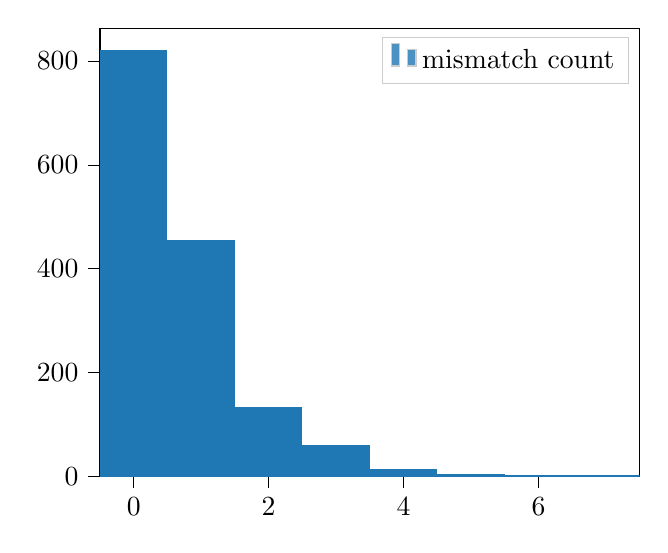
\begin{tikzpicture}

\definecolor{darkgray176}{RGB}{176,176,176}
\definecolor{lightgray204}{RGB}{204,204,204}
\definecolor{steelblue31119180}{RGB}{31,119,180}

\begin{axis}[
legend cell align={left},
legend style={fill opacity=0.8, draw opacity=1, text opacity=1, draw=lightgray204},
tick align=outside,
tick pos=left,
x grid style={darkgray176},
xmin=-0.5, xmax=7.5,
xtick style={color=black},
y grid style={darkgray176},
ymin=0, ymax=863.1,
ytick style={color=black}
]
\draw[draw=none,fill=steelblue31119180] (axis cs:-0.5,0) rectangle (axis cs:0.5,822);
\addlegendimage{ybar,ybar legend,draw=none,fill=steelblue31119180}
\addlegendentry{mismatch count}

\draw[draw=none,fill=steelblue31119180] (axis cs:0.5,0) rectangle (axis cs:1.5,455);
\draw[draw=none,fill=steelblue31119180] (axis cs:1.5,0) rectangle (axis cs:2.5,134);
\draw[draw=none,fill=steelblue31119180] (axis cs:2.5,0) rectangle (axis cs:3.5,61);
\draw[draw=none,fill=steelblue31119180] (axis cs:3.5,0) rectangle (axis cs:4.5,15);
\draw[draw=none,fill=steelblue31119180] (axis cs:4.5,0) rectangle (axis cs:5.5,5);
\draw[draw=none,fill=steelblue31119180] (axis cs:5.5,0) rectangle (axis cs:6.5,3);
\draw[draw=none,fill=steelblue31119180] (axis cs:6.5,0) rectangle (axis cs:7.5,3);
\end{axis}

\end{tikzpicture}
%
		}%
		\caption{128 bytes ($Pr[X=0] \approx 0.55$)}%
	\end{subfigure}%
	\begin{subfigure}{.5\textwidth}%
		\centering%
	    \resizebox{0.8\linewidth}{!}{%
			% This file was created with tikzplotlib v0.10.1.
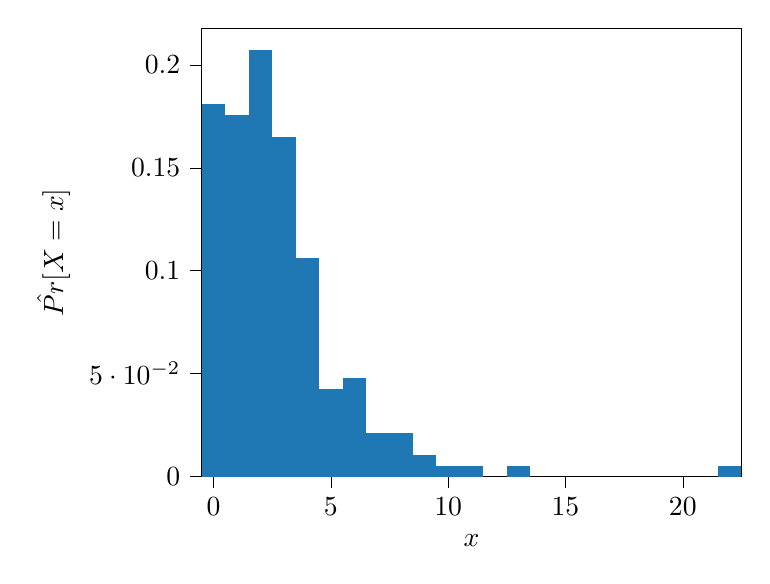
\begin{tikzpicture}

\definecolor{darkgray176}{RGB}{176,176,176}
\definecolor{steelblue31119180}{RGB}{31,119,180}

\begin{axis}[
tick align=outside,
tick pos=left,
x grid style={darkgray176},
xlabel={\(\displaystyle x\)},
xmin=-0.5, xmax=22.5,
xtick style={color=black},
y grid style={darkgray176},
ylabel={\(\displaystyle \hat{Pr}[X=x]\)},
ymin=0, ymax=0.21781914893617,
ytick style={color=black}
]
\draw[draw=none,fill=steelblue31119180] (axis cs:-0.5,0) rectangle (axis cs:0.5,0.180851063829787);
\draw[draw=none,fill=steelblue31119180] (axis cs:0.5,0) rectangle (axis cs:1.5,0.175531914893617);
\draw[draw=none,fill=steelblue31119180] (axis cs:1.5,0) rectangle (axis cs:2.5,0.207446808510638);
\draw[draw=none,fill=steelblue31119180] (axis cs:2.5,0) rectangle (axis cs:3.5,0.164893617021278);
\draw[draw=none,fill=steelblue31119180] (axis cs:3.5,0) rectangle (axis cs:4.5,0.106382978723405);
\draw[draw=none,fill=steelblue31119180] (axis cs:4.5,0) rectangle (axis cs:5.5,0.042553191489362);
\draw[draw=none,fill=steelblue31119180] (axis cs:5.5,0) rectangle (axis cs:6.5,0.0478723404255322);
\draw[draw=none,fill=steelblue31119180] (axis cs:6.5,0) rectangle (axis cs:7.5,0.021276595744681);
\draw[draw=none,fill=steelblue31119180] (axis cs:7.5,0) rectangle (axis cs:8.5,0.021276595744681);
\draw[draw=none,fill=steelblue31119180] (axis cs:8.5,0) rectangle (axis cs:9.5,0.0106382978723405);
\draw[draw=none,fill=steelblue31119180] (axis cs:9.5,0) rectangle (axis cs:10.5,0.00531914893617025);
\draw[draw=none,fill=steelblue31119180] (axis cs:10.5,0) rectangle (axis cs:11.5,0.00531914893617025);
\draw[draw=none,fill=steelblue31119180] (axis cs:11.5,0) rectangle (axis cs:12.5,0);
\draw[draw=none,fill=steelblue31119180] (axis cs:12.5,0) rectangle (axis cs:13.5,0.00531914893617025);
\draw[draw=none,fill=steelblue31119180] (axis cs:13.5,0) rectangle (axis cs:14.5,0);
\draw[draw=none,fill=steelblue31119180] (axis cs:14.5,0) rectangle (axis cs:15.5,0);
\draw[draw=none,fill=steelblue31119180] (axis cs:15.5,0) rectangle (axis cs:16.5,0);
\draw[draw=none,fill=steelblue31119180] (axis cs:16.5,0) rectangle (axis cs:17.5,0);
\draw[draw=none,fill=steelblue31119180] (axis cs:17.5,0) rectangle (axis cs:18.5,0);
\draw[draw=none,fill=steelblue31119180] (axis cs:18.5,0) rectangle (axis cs:19.5,0);
\draw[draw=none,fill=steelblue31119180] (axis cs:19.5,0) rectangle (axis cs:20.5,0);
\draw[draw=none,fill=steelblue31119180] (axis cs:20.5,0) rectangle (axis cs:21.5,0);
\draw[draw=none,fill=steelblue31119180] (axis cs:21.5,0) rectangle (axis cs:22.5,0.00531914893617025);
\end{axis}

\end{tikzpicture}
%
		}%
		\caption{1024 bytes ($Pr[X=0] \approx 0.18$)}%
	\end{subfigure}%
	\caption{Token mismatch statistic when using Meteor to encode Shakespear's Hamlet blockwise. The x-axis shows the number of tokenization mismatches between the encoding and the decoding party for hiddentext blocks with size...}
	\label{fig:meteor-stats-mismatch-count}	
\end{figure}

\section{Algorithmic Reconstruction Of Token Candidates}
\label{sec:alg-rec-tok-candidates}

Unfortunately, with sub-word tokenization, the decoding party cannot decide which tokens have been sampled to generate the stegotext.
To allow successful decoding of ambiguously tokenized stegotexts, I will in this section introduce algorithms to detect and fix wrong tokenizations. 


For that we have to modify the encoding step of Meteor to detect and fix wrong tokenization.
Before encoding, split the message $m$ into blocks $m_i$ of length $\gamma$.
After each block $m_i$, add a marker or checksum $q_i = q(m_i)$ of length $\delta$ into the hiddentext, i.e. $q \colon \{ 0,1 \}^\gamma \rightarrow \{ 0,1 \}^\delta$.
This marker helps the decoder to decide if the decoding is still correct up to this point.
The marker $q_i$ can be a checksum of $m_i$ or a fixed marker.
By using markers, we introduce $\delta \cdot \frac{|m|}{\gamma}$ bits of overhead to the hiddentext.
The modified $Encode$ algorithm can be found at \autoref{alg:marked-encode}.

Now the decoding party has to verify that after each block $m_i$ of $\gamma$ bits, the marker $q(m_i)$ appears and is valid.
If not, a decoding error has occured in the stegotext.
The modified $Decode$ algorithm can be seen at \autoref{alg:marked-decode}.

\begin{Pseudocode}[float, caption={Marked Encode Algorithm}, label={alg:marked-encode}]
algorithm $MarkedEncode_{\mathcal{M}}^{\beta, \gamma}(k_{prg}, m, \mathcal{H}, q)$
	Output: Stegotext message $c$
	$c \leftarrow \epsilon,~ n \leftarrow 0$
	$m^* \leftarrow \epsilon,~ j \leftarrow 0$
	while $j < |m|$ do
		$m^* \leftarrow m^* || m_j$
		$j \leftarrow j + 1$
		if $j \equiv 0~ \pmod \gamma$
			$m^* \leftarrow m^* || q(m_j)$
	while $n < |m^*|$ do
		$mask \leftarrow PRG.Next(k_{prg})$
		$r \leftarrow m^*[n:n+\beta] \oplus mask$
		$c_i \leftarrow Sample_{\mathcal{M}}^\beta(\mathcal{H}, r)$
		$\mathcal{R} = Recover_{\mathcal{M}}^\beta(\mathcal{H}, c_i)$
		$n_i \leftarrow LenPrefix^\beta(\mathcal{R})$
		$c \leftarrow c || c_i, n \leftarrow n+n_i, \mathcal{H} \leftarrow \mathcal{H}||c_i$
	Output $c$
\end{Pseudocode}



\begin{Pseudocode}[float, caption={Marked Decode Algorithm}, label={alg:marked-decode}]
algorithm $MarkedDecode_{\mathcal{M}}^{\beta,\gamma}(k_{prg}, c, \mathcal{H}, q)$
	Output: Plaintext message $m$
	$m \leftarrow \epsilon,~ n \leftarrow 0,~ j \leftarrow 0$
	Parse $c$ as $\{ c_0, c_1, \dots, c_{|c|-1} \}$
	for $i \in \{0, 1, \dots, |c|-1 \}$ do
		$\mathcal{R} = Recover_{\mathcal{M}}^\beta(\mathcal{H}, c_i)$
		$n_i \leftarrow LenPrefix^\beta(\mathcal{R})$
		$n \leftarrow n + n_i$
		$j \leftarrow j + n_i$
		if $j \geq \gamma$
			$j \leftarrow j - \gamma$
			!!TODO!! fixme n is wrong here, need to track current index
			if $m[n:n+\gamma] \neq q(m_i)$ do
				rollback()
		$m_i \leftarrow Prefix^\beta(\mathcal{R})$
		$mask \leftarrow PRG.Next(k_{prg})$
		$m \leftarrow m || (m_i \oplus mask[0: |m_i|])$
		$\mathcal{H} \leftarrow \mathcal{H}||c_i$
	Output $m$
\end{Pseudocode}
\todo{Modify Decode to MarkedDecode}

For the modification above, we need a helper algorithm which generates all possible tokenizations for a given stegotext.
We can represent these tokenization candidates in a graph using the ML models's tokens $\mathcal{T}$.

When passed a string $c$, the algorithm \emph{TokenizeCandidates} generates a directed, acyclic graph (DAG) $G = (V, E)$.
The nodes $v \in V$ represent all possible suffix strings of $c$ with $|V| = |c| + 1$.
The edges $e \in E$ represent possible tokens to use to transition between suffixes.
An example graph for input ``hello'' can be found at \ref{fig:ex-graph-tokenize-candidates}.
For example, the suffix string ``ello'' can be transformed to ``lo'' by removing the token ``el''.

Now that we have a graph for $c$, we can generate every possible sequence of tokens which $c$ can be parsed as.
For that, we use the algorithm $AllPaths$, which takes as input a graph $G = (V, E)$ and a start node $v_i \in V$ and returns a set of all possible paths between $v_i$ and a sink node $v_j = \epsilon$.

But how many paths exist between $v_i$ and $v_j$? A path between $v_i$ and $v_j$ is a subset of $E$ which contains both $v_i$ and $v_j$.
In the worst case, $G$ is a DAG with $\frac{n(n-1)}{2}$ edges and $v_i = max_{topological}(V)$ and $v_j = min_{topological}(V)$.
There are at most $2^{|V|-2} = 2^{|c|-1}$ subsets of $E$ which contain both $v_i$ and $v_j$.
The output of $AllPaths$ is exponential in input length.
A DFS-based implementation for AllPaths can be found at \autoref{alg:all-paths}.

\begin{Pseudocode}[float,caption={TokenizeCandidates algorithm},label={alg:tokenize-candidates}]
	algorithm $TokenizeCandidates_{\mathcal{T}}(s)$
		Output: Graph $G = (V, E)$
		if $s = \epsilon$
			return $\epsilon$
		for $t \in \mathcal{T}$ do
			if $s[0{:}|t|] = t$ do
				$V \leftarrow V \cup \{ s[|t|{:}] \}$
				$E \leftarrow E \cup \{ (s, s[|t|{:}]) \}$
				$G \leftarrow G \cup TokenizeCandidates_{\mathcal{T}}(s[|t|{:}])$
		return $G$
\end{Pseudocode}

\begin{figure}[htbp]
	\centering
	\begin{tikzpicture}
		\node[block] (hello) {hello};
		\node[block, right=15mm of hello] (lo) {lo};
		\node[block, above=15mm of lo] (llo) {llo};
		\node[block, above=15mm of llo] (ello) {ello};
		\node[block, below=15mm of lo] (o) {o};
		\node[block, right=15mm of lo] (bot) {$\epsilon$};
		
		\draw[->] (hello) to node[above] {h} (ello);
		\draw[->] (hello) to node[above] {he} (llo);
		\draw[->] (hello) to node[above] {hel} (lo);
		\draw[->] (hello) to node[left] {hell} (o);
		\draw[->, bend right=120] (hello) to node[below] {hello} (bot);

		\draw[->] (ello) to node[right] {e} (llo);
		\draw[->, bend left=30] (ello) to node[right] {el} (lo);
		\draw[->, bend left=30] (ello) to node[above] {ell} (o);
		\draw[->] (ello) to node[right] {ello} (bot);

		\draw[->] (llo) to node[right] {l} (lo);
		\draw[->, bend right=30] (llo) to node[above] {ll} (o);
		\draw[->] (llo)   to node[above] {llo} (bot);

		\draw[->] (lo)    to node[right] {l} (o);
		\draw[->] (lo)    to node[above] {lo} (bot);

		\draw[->] (o)     to node[above] {o} (bot);
	\end{tikzpicture}
	\caption{
Graph generated by $TokenizeCandidates_{\mathcal{T}}(``hello'')$ with $\mathcal{T} = \{ h, e, l, l, o, el, he, ll, lo, ell, hel, llo, hell, ello, hello \}$.
The nodes in the graph represent substrings of $s = $``hello'' which are accessible by removing a prefix token $t \in \mathcal{T}$ from $s$.
The edges are labeled with the token used to transform the left-hand side node to the right-hand side node.
The special node $\epsilon$ represents the empty string and is a sink in the graph.
The list of all possible paths between $s$ and $\epsilon$ are the possible tokenizations of $s$ using tokens $\mathcal{T}$.
}
	\label{fig:ex-graph-tokenize-candidates}
\end{figure}
\todo{improve tikz graph}

\begin{Pseudocode}[float,caption={DFS-based algorithm which generates a list of all possible paths between between two nodes in a DAG},label={alg:all-paths}]
algorithm $AllPaths(G, root, sink)	$
	Output: List of paths between $root$ and $sink$
	if $root = sink$ do
		return $[[\bot]]$
	$queue \leftarrow \epsilon$
	$paths \leftarrow []$
	$hops \leftarrow OutEdges(G, root)$
	$queue \leftarrow queue + hops$
	for $hop \in hops$ do
		$subpaths \leftarrow AllPaths(G, hop, sink)$
		for $subpath \in subpaths$ do
			$paths \leftarrow [[root] + subpath]$
	return $paths$
\end{Pseudocode}
\todo{improve performance using dynamic programming}
\chapter{Two-Way Communication}
\label{chap:twowaycommunication}


In the Prisoners' Problem \cite{Simmons1983}, a unidirectional channel is described.
The sending party Alice embeds a hidden message in a cover channel, the receiving party Bob decodes the received message.
The Meteor stegosystem adopts this approach of receiving and sending parties.
But in most practical applications, a bidirectional communication channel between participants is needed.
For example in client-server architectures such as HTTP or key exchange protocols such as Diffie-Hellman, the participants exchange messages bi-directionally.
Also, one of the most commonly used mediums for text messages is instant messaging, which is characterized by a continuous back-and-forth of messages between participants.

Since the Meteor stegosystem is constructed to be very adaptable to different underlying distributions (as long as they are RRRSS), we can modify Meteor to generate stegotext messages for use in the context of instant messaging.
In this chapter, we will introduce a simple protocol for two-way communication using Meteor and adapt Meteor to use DialoGPT \cite{Zhang2020}, a GPT-based generative model which is trained to generate text messages as they could appear in a chat.

\section{Protocol for Two-Way Communication}

In \autoref{fig:twowaycommunication}, we introduce a simple chat protocol between two participants Alice and Bob.
Here, Alice and Bob send messages back and forth.
Alice sends stegotext blocks, while Bob generates a sequence of responses, which can be stegotexts or handwritten messages.
After each message from Alice, Bob uses the Meteor stegosystem to decode $s_i$ to a message block $m_i$.
After $\ell$ iterations, the entire stegotext has been sent.
Now, Bob can recover the hiddentext $m$ by concatenating the decoded blocks $m_i$.


\begin{figure}[htbp]
  \centering
  \begin{msc}[instance distance=4cm,action width=5cm]{Two-Way Steganographic Communication Protocol}
    \declinst{alice}{}{Alice}
    \declinst{bob}{}{Bob}
    \condition{exchange key $k$ and history $h$}{alice,bob}
    \nextlevel[2]
    \action{split hiddentext $m$ in $\ell$ blocks $m_i$}{alice}
    \nextlevel[3]
    \condition{for $i \in \{ 1, 2, \dots, \ell \}$ do}{alice,bob}
    \nextlevel[2]
    \action{$s_i = Encode_{\mathcal{C}}^\beta(m_i, k, h)$}{alice}
    \nextlevel[3]
    \mess{$s_i$}{alice}{bob}
    \nextlevel
    \action{$m_i = Decode_{\mathcal{C}}^\beta(s_i, k, h)$}{bob}
    \nextlevel[2]
    \action{Generate response $r$}{bob}
    \nextlevel[3]
    \mess{$r$}{bob}{alice}
    \nextlevel
    \action{$h \leftarrow h || r$}{alice}
    \action{$h \leftarrow h || r$}{bob}
    \nextlevel[2]
    \condition{endfor}{alice,bob}
    \nextlevel[3]
    \action{$m = m_1 || m_2 || \dots || m_{\ell}$}{bob}
    \nextlevel
  \end{msc}
  \caption{
  A Two-Way Steganographic Communication Protocol for participants Alice and Bob.
  In this scheme, Alice encodes blocks of her hiddentext message $m$ into stegotexts $s_i$ and sends them to Bob, who decodes the blocks using the Meteor stegosystem.
  Bob then generates his response $r$ and sends it back.
  The response can be generated using a GNN, be (part of) a stegotext, or handwritten chat messages.
  After $\ell$ iterations, Bob can reconstruct the hiddentext $m$ by concatenating the $m_i$.
  }
  \label{fig:twowaycommunication}
\end{figure}

\section{Implementation of Two-Way Communication}
While we can generate stegotexts for two-way communication using the GPT-2 model, as the original Meteor stegosystem does, the texts generated with GPT-2 are not convincing as chat messages. 
In the following example, we see a conversation between Alice and Bob using the protocol described in \autoref{fig:twowaycommunication}.
The initial history consists of a short sequence of messages where both participants greet and ask each other how their respective day was.
Alice's messages encode the hiddentext ``Hi there!'' in blocks of 32 bits, while Bob's responses are generated manually.

\begin{example}[Meteor Conversation for hiddentext ``Hi there!'' using GPT-2 with 32 bit blocksize]
\leavevmode
\begin{itemize}
\item Alice: I've been trying to get my hands on a couple of these since they were first released last year, and it's been a fun time. It's been a long time since I've had the chance to play through
\item Bob: What games do you like to play?
\item Alice: "It's a long haul, but it's a long haul," said Steve Young, the former director of the FBI's counter
\item Bob: Are you affiliated with the FBI?
\item Alice: How To Use
\end{itemize}
\end{example}

As we can see, the generated text does not read as if it was an actual conversation between friends.
Also, the generated texts appear to lack context.
Alice's texts don't seem to take Bob's responses into account and cover quite different topics in each iteration.
This effect is due to the nature of GPT's training dataset called WebText, which is a large undisclosed collection of online newspaper articles, books, blog posts, and the like.
Therefore, it is very likely that GPT generates probability distributions for article-like texts.
When sampling from these distributions, it is likely to generate text that reads like a newspaper article as well.

Fortunately, the NLP community is very active in building different models for many use cases.
In 2019, DialoGPT, a pre-trained transformer trained on public multi-turn dialogues from Reddit threads, has been published \cite{Zhang2020}.
As the name suggests, DialoGPT is a derivation of GPT that is trained and fine-tuned for dialogue generation.
When repeating the same experiment as above, but with the DialoGPT model as a drop-in replacement for GPT-2, the results read more like what we would expect from a chat conversation between friends.
Again, Alice's text messages encode the hiddentext ``Hi there!'' with 32 bits of encoded data per chat message.
Bob's responses are handwritten.
While a little bit incoherent, the transcript is closer to an actual conversation between friends.

\begin{example}[Meteor Conversation for hiddentext ``Hi there!'' using DialoGPT with 32 bit blocksize]
\leavevmode
\begin{itemize}
\item Alice: I suppose it is . I'm a bit jealous of the weather today , though . It's nice , but it's nice to be in a nicer
\item Bob:   I don't know, it's too hot for me today to be honest :D
\item Alice: Yeah it is . I wish it was cooler though . I love it here . I wish I had another place to live though . We're all pretty cool here . Lol
\item Bob:   haha you're cool for sure
\item Alice: I love it here as
\item Bob:   Where are you currently?
\end{itemize}


\end{example}
\chapter{Security Analysis}
\label{chap:security}

When we communicate using a steganographic protocol, secrecy is of upmost importance.
We probably communicate in an environment which is very hostile against its communication participants.
Therefore, we should satisfy the most rigorous security requirements we can possibly satisfy.

In \autoref{chap:previous-work}, we have discussed two different definitions of steganographic secrecy.
In \autoref{def:sec-kaptchuk}, we have seen a rigorous definition of steganographic secrecy when we defined \emph{steganographic secrecy against chosen hiddentext attacks}, or SS-CHA.
Later, in \autoref{sec:meteor}, we have introduced the Meteor stegosystem and its definition of security.
In this chapter, we will
\begin{itemize}
	\item compare Meteor's security definition with Hopper's security game,
	\item show that the Meteor stegosystem does not satisfy Hopper's security game,
	\item modify Meteor to improve its security against SS-CHA adversaries.
\end{itemize}

\section{Comparison Of Meteor's And Hopper's Security Game}

In \autoref{sec:prov-sec-steg} and \autoref{sec:meteor}, we have discussed Hopper's and Meteor's definition of steganographic secrecy against chosen hiddentext attackers. 
In this section, we will compare the security definition of the Meteor stegosystem with Hopper's definition of SS-CHA and see that Meteor's definition is weaker than Hopper's.

In \autoref{def:sec-kaptchuk}, it is argued that a stegosystem is secure against chosen hiddentext attack, if for all $k \leftarrow KeyGen(1^\lambda)$, the probability of an attacker to distinguish an output of $Encode(k, \cdot, \cdot)$ from the output of a random oracle $\mathcal{O}(\cdot, \cdot)$ is negligible in $\lambda$. In Meteor's security proof, it is argued that Meteor satisfies this security definition by reduction to the underlying PRG.

\begin{theorem}
	Meteor is secure (\autoref{def:sec-kaptchuk}) against ppt. adversaries. 
\label{thm:meteor-secure}
\end{theorem}
\begin{proof}
	Let $\mathcal{A}$ be an attacker against the Meteor stegosystem, i.e. $\mathcal{A}$ can distinguish outputs of $Encode$ from those of a random oracle $\mathcal{O}$. 
	We will now show that $\mathcal{A}$ is also an attacker against the underlying PRG.
	The attacker only sees the outputs $c = c_0 ||c_1 || \dots || c_{\tau}$ of $Encode$ and $\mathcal{O}$, respectively.
	When we take a look at the implementation of $Encode$, we observe that the only output difference to $\mathcal{O}$ in the view of the attacker is the randomness $r$ used to sample $c_i$ from the underlying distribution.
	
	How is $r$ constructed? 
	It is the exclusive-or of $\beta$ bits of $m$ and a pseudorandom value $mask$ from PRG.
	Since $mask$ is a output of a pseudorandom generator which we expect to be indistinguishable from true randomness, the exclusive or of $mask$ with some other value is indistinguishable from true randomness as well.
	But to distinguish the output of $Encode$ from some oracle $\mathcal{O}$, the attacker has to distinguish $r$ from a randomly sampled token, i.e. the attacker has to distinguish $r$ from a truly random value $r'$.
	
	Therefore, $\mathcal{A}$ can be used to attack the PRG.
	Since we expect the underlying PRG to be secure, $\mathcal{A}$ cannot distinguish $r$ from $r'$ with non-negligible probability in polynomial time.
\end{proof}

But is this sufficient to satisfy Hopper's definition of steganographic secrecy?
Unfortunately not.
In Hopper's $(t,q,l)$-SS-CHA game, an attacker may perform up to $q(k)$ queries.
The aforementioned security proof only considers security against one query.
If $\mathcal{A}$ repeats the same query twice, the Meteor system will return the same output, while $\mathcal{O}$ will~ --~ with overwhelming probability~ --~ sample an entirely different sequence from the distribution.
After only two queries, $\mathcal{A}$ is able to distinguish Meteor's outputs from those of a random oracle with high certainty.


\section{Improve Meteor's Security}

To improve Meteor's security, we have to randomize the output of $Encode$, i.e. on each invocation with the same inputs, $Encode$ should, with high probability, return a different stegotext, while retaining indistinguishability from random sampling.

To achieve that we have to introduce a new cryptographic primitive, symmetric encryption schemes (SES) in counter (CTR) mode based on a pseudorandom function (PRF) $F$.
We introduce a definition of a SES in Figure \ref{fig:ses} which is a simplified variant of that introduced in \cite{Berndt2017}.
There, it is argued that SES satisfies the IND\$-CPA property if F is a secure pseudorandom function.

The idea behind encryption in SES-CTR is simple:
First, split the message $m$ into $n$ blocks of size $F.in(\lambda)$ specific to $F$.
Secondly, choose an $IV$ of size $F.in(\lambda)$ at random.
It is important to not reuse an $IV$ with a given key $k$ to retain One-Time-Pad security.
Now, for each block $m_i$, use $F.Eval$ to generate the pseudorandom value $r = F.Eval(k, IV+i)$.
Afterwards, calculate the exclusive or of $r$ and $m_i$ to get the next block $c_i$.
The ciphertext of size $(n+1)\cdot F.in(\lambda)$ is the IV concatenated with ciphertext blocks $c_i$.

Decryption is similar to encryption.
First, split $c$ in $n+1$ blocks of size $F.in(\lambda)$.
Interpret the first block of $c$ as $IV$.
Afterwards, analogously to encryption, for each block $c_i$, calculate $r = F.Eval(k, IV+i)$.
Now, calculate the exclusive or of $r$~ and $c_i$ to recover the message block $m_i = c_i \oplus r$.

Now that we have established the concept of an SES, we still need to find $F$ which is a PRF.
In practice, we can use AES as $F$, which is believed to be a pseudorandom permutation (PRP), with key $k$ and messages $IV+i$.

\begin{figure}[htbp]%
	\centering%
	\begin{Pseudocode}
algorithm $SES.Encrypt_F(k, m=m_1 m_2 \dots m_n \in \{0,1\}^{n\cdot F.in(\lambda)})$
	Output: Ciphertext $c$
	$\lambda = |k|$
	$IV \leftarrowS \{0,1\}^{F.in(\lambda)}$
	for $i \in \{ 1, 2, \dots, n \}$ do
		$c_i \leftarrow F.Eval(k, (IV+i) \mod 2^{F.in(\lambda)}) \oplus m_i$
	Output $IV||c_1||c_2||\dots||c_n$
	\end{Pseudocode}%
	\begin{Pseudocode}
algorithm $SES.Decrypt_F(k, c=c_0 c_1 \dots c_n \in \{0,1\}^{(n+1)\cdot F.in(\lambda)})$
	Output: cleartext $m$
	$\lambda = |k|$
	$IV \leftarrow c_0$
	for $i \in \{ 1, 2, \dots, n \}$ do
		$m_i \leftarrow F.Eval(k, (IV+i) \mod 2^{F.in(\lambda)}) \oplus c_i$
	Output $m_1||m_2||\dots||m_n$
	\end{Pseudocode}%
	\caption{Symmetric Encryption Scheme (SES) in counter (CTR) mode}%
	\label{fig:ses}%
\end{figure}%


In \autoref{alg:encode-nd}, we prepend the bits encoded in the covert distribution with an initialization vector IV randomly sampled from bitstrings of length $\gamma$.
This IV is then used as randomness input for our PRF.
Since IV is pseudorandom, an attacker cannot distinguish the sampled tokens from those sampled by a random oracle $\mathcal{O}$.

\autoref{alg:encode-nd} and \autoref{alg:decode-nd} improve Meteor's steganographic secrecy.
The algorithms use the SES scheme defined above, replacing the original One-Time-Pad based encryption scheme.
Since SES is IND\$-CPA secure we can, with the same reduction as in Theorem \ref{thm:meteor-secure}, show SS-CHA secrecy against polynomial attackers as long as the same $IV$ is not encountered twice, which is -- in practice -- very unlikely for sufficient IV lengths.


\begin{Pseudocode}[float, caption={
Meteor EncodeRandomized Algorithm.
This algorithm differs from the original Encode algorithm by using a SES to encrypt the message.
The ciphertext (which is indistinguishable from randomness) is then used to sample from $\mathcal{M}$.
}, label={alg:encode-nd}]
algorithm $EncodeRandomized_{\mathcal{M}}^{\beta}(k_{prg}, m, h)$
	Output: Stegotext message $c$
	$c \leftarrow \epsilon,~ j \leftarrow 0,~ n \leftarrow 0$
	$r \leftarrow SES.Encrypt(k, m)$
	while $n < |r|$ do
		$c_i \leftarrow Sample_{\mathcal{M}}^\beta(h, r[n: n+\beta])$
		$\mathcal{R} \leftarrow Recover_{\mathcal{M}}^\beta(h, c_i)$
		$n_i \leftarrow LenPrefix^\beta(\mathcal{R})$
		$c \leftarrow c || c_i, n \leftarrow n+n_i, h \leftarrow h||c_i$
	Output $c$
\end{Pseudocode}
\begin{Pseudocode}[float, caption={
Meteor DecodeRandomized Algorithm.
This algorithm differs from the original Decode algorithm by interpreting the first $\gamma$ bits of the hiddentext as IV.
After decoding $\gamma$ bits of hiddentext, a PRF is initialized with IV for generation of pseudorandom masks.}, label={alg:decode-nd}]
algorithm $DecodeRandomized_{\mathcal{M}}^{\beta}(k_{prg}, c, h)$
	Output: Plaintext message $m$
	$m \leftarrow \epsilon,~ n \leftarrow 0,~ r \leftarrow \epsilon$
	Parse $c$ as $c_0 || c_1 || \dots || c_{\tau}$
	for $i \in \{ 0, 1, \dots, \tau \}$ do
		$\mathcal{R} \leftarrow Recover_{\mathcal{M}}^\beta(h, c_i)$
		$r_i \leftarrow Prefix^\beta(\mathcal{R})$
		$r \leftarrow r || r_i$
		$h \leftarrow h||c_i$
	$m \leftarrow SES.Decrypt(k, r)$
	Output $m$
\end{Pseudocode}
\chapter{Conclusion}
\label{chap:conclusion}

We have discussed Meteor, an innovative stegosystem that uses generative neural networks to embed a hiddentext into a covert channel.
It achieves that by replacing the randomness used for sampling with an encryption of the hiddentext.

If the encrypted hiddentext is indistinguishable from randomness, this process is secure against chosen hiddentext attackers.
In \autoref{chap:security}, we have seen that this is the case if an attacker is allowed to send up to one query in the SS-CHA game.
Unfortunately, Meteor's security guarantee does not hold for attackers who can send polynomial queries, because Meteor's output is deterministic.
To fix this, we discussed a modification to Meteor that uses a symmetric encryption scheme (SES) in counter mode to become indeterministic while maintaining indistinguishability from randomness.

We have also modified Meteor for two-way communication for use in the context of instant messaging in \autoref{chap:twowaycommunication}.
To use Meteor in instant messaging, the hiddentext is split into blocks to generate shorter stegotext messages.
While the texts generated by GPT-2 are not very convincing as chat messages, we can easily adapt Meteor to use other GNN models, as long as they satisfy the RRRSS property defined in \autoref{def:rrrss}.
We adapted Meteor to use the DialoGPT model.
The stegotexts generated with the DialoGPT model more closely resemble those found in instant messaging.

We also found that Meteor sometimes generates stegotexts that cannot be decoded correctly in \autoref{chap:correctness}.
These decoding errors happen more frequently the longer the hiddentext is.
This problem occurs due to subword tokenization, a feature of modern GNNs which greatly increases model performance.
We have discussed a modification to the Meteor stegosystem which fixes these decoding errors while -- in the worst case and for some models -- introducing computational decoding overhead exponential in stegotext length.
This modification first tries to detect a decoding error with a checksum of length $\delta$ for message blocks of length $\gamma$ and, in case a decoding error occurs, generates every possible tokenization of a part of the stegotext.
Further research could compare different values for $\gamma$ and $\delta$ to find a good trade-off between stegotext length and computational overhead or develop more efficient techniques to recover from decoding errors.

While the Meteor authors have discussed that the Meteor stegosystem will be adaptable to GPT-3 once it is released, OpenAI unfortunately did not yet decide to release their model publicly and only allows limited access to GPT-3 using a private (and paid) online API.
While it would technically still be possible to use this private API with Meteor, its practical use in a stegosystem is limited.
Also, the occurring costs of US\$ 1.12 to US\$ 55.92 per megabyte of hiddentext (US\$ 0.0004 to US\$ 0.02 per 1000 tokens with an average of 3 bits of hiddentext per token) are a problem in practical use \cite{OpenAIPricing2022}.

Fortunately, researchers have built and trained open source alternatives to GPT-3.
One alternative might be GPT-NeoX, a generative model with 20 billion parameters that can arguably compete with GPT-3 in prediction quality \cite{GPTneo2022}.
Also, GPT-NeoX seems to be compatible with GPT-2, since it uses the same tokenizer and token dictionary.
Further research could incorporate GPT-NeoX as an alternative model for use with the Meteor stegosystem.
First experiments conducted for this thesis have concluded that text generation with large models, i.e. models with parameters an order of magnitude greater than GPT-2's 345 million parameters, requires a considerable amount of computational power which state-of-the-art laptops cannot deliver without hardware acceleration.

Another promising topic for further research could be to adapt the Meteor stegosystem to use public keys instead of symmetric keys and allow steganographic group communication.

The Meteor stegosystem establishes a very promising approach for using generative neural networks in cryptographically secure steganographic systems.
Since it can be expected that computational performance in machine learning will continue to improve in the coming years, steganography on ML models is likely to remain a promising area of research.

\end{document}

%  LocalWords:  LaTeX tex moretexcs Lübeck pdf uzl lualatex bibtex th
%  LocalWords:  TechReport Kernighan Lamport's Tantau's Tantau cls kZ
%  LocalWords:  Mustermann emacs oldschool pdflatex texmf utf biber
%  LocalWords:  biblatex Alphabetische Bibliographie Numerische VIIa
%  LocalWords:  varioref german Einleitung Beiträge dieser Arbeit xml
%  LocalWords:  Ergebnisse Verwandte Arbeiten Aufbau nucleotide VIIc
%  LocalWords:  ensembl amino phylogenetic Alexa Siri decrypt versa
%  LocalWords:  cryptographic pre nondeterministic deterministically
%  LocalWords:  Beutelspacher Untersuchungen zum genetischen sep llcc
%  LocalWords:  Beispiel tikz jpg png Alegrya Kasimir Malewitsch PGF
%  LocalWords:  Lamport Institut für Theoretische Informatik zu url
%  LocalWords:  Universität Springer DowneyF Downey Parameterized doi
%  LocalWords:  BibLaTeX Kime Philipp urldate Mittelbach hyperref Lua
%  LocalWords:  Rahtz Oberdiek Heiko Braams Bezos López fontspec Das
%  LocalWords:  Arseneau amsmath ist Tipps und zur Formulierung
%  LocalWords:  mathematischer Gedanken Mathematik Studienanfänger
%  LocalWords:  Albrecht Vieweg Teubner Verlag
